% !TeX program = xelatex
\documentclass{article}

\usepackage{xeCJK}
\usepackage{listings}
\usepackage{graphicx}
\usepackage{geometry}
\usepackage{hyperref}
\usepackage{tabularx}
\usepackage{afterpage}
\usepackage{tcolorbox}
\setCJKmainfont{Noto Sans Mono CJK TC} % 設定中文字體
\setCJKmonofont{Noto Sans Mono CJK TC}
\geometry{a4paper, left=2cm, right=2cm, top=2cm, bottom=2cm}
\hypersetup{
    colorlinks=true,    % 将书签文字用颜色表示
    linkcolor=blue,     % 内部链接的颜色
    citecolor=green,    % 引用的颜色
    filecolor=magenta,  % 文件链接的颜色
    urlcolor=cyan       % URL的颜色
}
\lstset{
    language=Python,
    basicstyle=\ttfamily\small,
    commentstyle=\color{green!40!black},
    keywordstyle=\color{blue},
    numbers=left,
    numberstyle=\tiny\color{gray},
    stepnumber=1,
    numbersep=5pt,
    backgroundcolor=\color{gray!10},
    frame=single,
    rulecolor=\color{black!30},
    breaklines=true,
    breakatwhitespace=true,
    showspaces=false,
    showstringspaces=false,
    showtabs=false,
    tabsize=4,
    captionpos=b,
    frame=tb
}



\title{ROS 筆記}
\author{luu}
\date{} % 添加日期

\begin{document}

\maketitle
\tableofcontents


\clearpage
\part{ros2入門CLI操作}
接下來的資料來源於ros官方文件,可以上去看看。
\href{https://docs.ros.org/en/humble/Installation.html}{ros2}
\section{CLI 設定}
% cli_settings.tex
在運行ROS 2的指令時需要開啟環境,所以要先使用source來啟用。
\begin{verbatim}
source /opt/ros/humble/setup.zsh
\end{verbatim}
但是每次都要執行會有點多餘,所以可以寫在shell的設定檔內。
\begin{verbatim}
echo "source /opt/ros/humble/setup.zsh" >> ~/.zshrc
\end{verbatim}


\section{練習用的模擬器}
% simulator_practice.tex
Turtlesim是一個用於學習ROS 2的輕量級模擬器。它說明了ROS 2在最基本層面上的功能,讓您了解稍後將使用真實機器人或機器人模擬做什麼。

ROS 2工具是使用者管理、反思以及與ROS系統互動的方式。它支援針對系統及其操作的不同方面的多個命令。人們可以使用它來啟動節點、設定參數、監聽主題等等。ROS 2工具是核心ROS 2安裝的一部分。

\subsection*{安裝}
安裝東西的時候記得要更新來源。
\begin{verbatim}
sudo apt update
sudo apt install ros-humble-turtlesim
sudo apt install ~nros-humble-rqt"*
\end{verbatim}
檢查軟體包是否已安裝:
\begin{verbatim}
ros2 pkg executables turtlesim
#--------------------
turtlesim draw_square
turtlesim mimic
turtlesim turtle_teleop_key
turtlesim turtlesim_node
\end{verbatim}

\subsection*{運行}
烏龜模擬器
\begin{verbatim}
ros2 run turtlesim turtlesim_node
ros2 pkg executables turtlesim
\end{verbatim}

rqt是ROS 2的圖形使用者介面(GUI)工具。在rqt中完成的所有操
作都可以在命令列上完成,但rqt提供了一種更用戶友好的方式來操作ROS
2元素。
\begin{verbatim}
rqt
\end{verbatim}


\section{節點}
ROS 中的每個節點都應負責單一的模組化目的,例如控制車輪馬達或發布來自雷射測距儀的感測器資料。每個節點都可以透過主題、服務、操作或參數從其他節點發送和接收資料。

完整的機器人系統由許多協同工作的節點組成。在 ROS 2 中,單一可執行檔(C++ 程式、Python 程式等)可以包含一個或多個節點。

\subsection{ros2 直行方法}
run 的使用方式如下
\begin{verbatim}
    ros2 run <package_name> <executable_name>
    -------------------------------------------
    usage: ros2 run [-h] [--prefix PREFIX]
    package_name executable_name ...

    Run a package specific executable

    positional arguments:
    package_name     Name of the ROS package
    executable_name  Name of the executable
    argv             Pass arbitrary arguments to the executable

    options:
    -h, --help       show this help message and exit
    --prefix PREFIX  Prefix command, which should go before the
    executable. Command must be wrapped in quotes
    if it contains spaces (e.g. --prefix 'gdb -ex
    run --args').
\end{verbatim}
操作流程如下
\begin{enumerate}
    \item 開啟第一個terminal
    \item 開啟turtlesim turtlesim\_node
    \item 開啟第二個terminal
    \item 檢查節點裝況
\end{enumerate}
開啟模擬視窗
\begin{verbatim}
    ros2 run <package_name> <executable_name>
    ros2 run turtlesim turtlesim_node
\end{verbatim}

檢查節點
\begin{verbatim}
    ros2 node list
\end{verbatim}
開啟控制器
\begin{verbatim}
    ros2 run turtlesim turtle_teleop_key
\end{verbatim}
\subsection{重新映射}
重新映射可讓您將預設節點屬性(例如節點名稱、主題名稱、服務名稱等)重新指派給自訂值。
\begin{verbatim}
ros2 run turtlesim turtlesim_node --ros-args --remap \
__node:=my_turtle
\end{verbatim}
這時後會看到我們映射的節點
\begin{verbatim}
    /my_turtle
    /turtlesim
    /teleop_turtle
\end{verbatim}

\subsection{節點訊息}
    可以用info 來查詢節點的資料,方法如下。
\begin{verbatim}
ros2 node info <node_name>
ros2 node info /my_turtle
\end{verbatim}
可以看到如下的連線資料
\begin{enumerate}
    \item  Subscribers:訂閱者
    \item  Publishers:發布者
    \item  Service Servers:服務伺服器
    \item  Service Clients:服務客戶端
    \item  Action Servers:動作伺服器
    \item  Action Clients:動作客戶端
\end{enumerate}
\subsubsection{訂閱者(Subscribers):}

訂閱者是ROS中的一個元件,它可以接收特定主題(Topic)的訊息。
主題是ROS中一種訊息傳遞機制,允許節點(ROS中的程式)透過發佈和訂閱訊息進行通訊。
\subsubsection{發佈者(Publishers):}

發佈者是ROS中的一個元件,它能夠向特定主題發佈訊息。
發佈者節點生成訊息並將其發送到相應的主題,使其他訂閱者節點能夠接收這些訊息。
\subsubsection{服務伺服器(Service Servers):}

服務伺服器提供了一種不同的通訊機制,稱為服務(Service),允許節點提供某種特定的功能或服務。
當一個節點請求服務時,服務伺服器執行相應的任務,並返回結果。
\subsubsection{服務客戶端(Service Clients):}

服務客戶端是一個節點,它能夠向服務伺服器發送請求,並等待伺服器返回結果。
這種通訊模式通常用於需要特定服務或功能的節點之間的交互。
\subsubsection{動作伺服器(Action Servers):}

動作伺服器是ROS中處理長時間執行任務的一種機制。它允許異步執行,並提供反饋。
與服務不同,動作可以週期性地提供反饋,而不僅僅是單一的請求和回應。
\subsubsection{動作客戶端(Action Clients):}

動作客戶端是一個節點,它可以向動作伺服器發送請求,並接收反饋和結果。
這通常用於需要處理較長時間執行的任務,而服務模型則適用於簡短的請求和回應。

\section{主題}
\subsection{topic 用法}
主題是在節點之間以及系統不同部分之間移動數據的主要方式之一。

可以用-h來查詢topic可以有哪些操作如下。
\begin{enumerate}
\item  bw     :顯示主題使用的頻寬
\item  delay  :從標題中的時間戳顯示主題的延遲
\item  echo   :從主題輸出訊息
\item  find   :輸出給定類型的可用主題列表
\item  hz     :將平均發布平率列印到螢幕上
\item  info   :列印主題的訊息
\item  list   :輸出可用主題的列表
\item  pub    :向主題發布訊息
\item  type   :列印主題的類型
\end{enumerate}

\subsection{list}
在新終端機中執行該命令將傳回系統中目前活動的所有主題的清單:
 \begin{verbatim}
     ros2 topic list 
     ----------------
     /parameter_events
     /rosout
     /turtle1/cmd_vel
     /turtle1/color_sensor
     /turtle1/pose
\end{verbatim}

\subsection{echo}
若要查看某個主題上發布的數據,請使用:

 \begin{verbatim}
     ros2 topic echo <topic_name>
     ros2 topic echo /turtle1/cmd_vel
     ---------------------------------
     linear:
     x: 2.0
     y: 0.0
     z: 0.0
     angular:
     x: 0.0
     y: 0.0
     z: 0.0
     ---
\end{verbatim}
\subsection{info}
可以查詢主題的訂閱與發布資訊。
\begin{verbatim}
    ros2 topic info /turtle1/cmd_vel
    --------------------------------
    Type: geometry_msgs/msg/Twist
    Publisher count: 1
    Subscription count: 2
\end{verbatim}

\subsection{interface}
節點使用訊息透過主題發送資料。發布者和訂閱者必須發送和接收相同類型的訊息才能進行通訊。

我們可以透過info去查詢topic的tyep,在由interface show 來查詢格式。

\newpage
\begin{verbatim}
    ros2 interface show geometry_msgs/msg/Twist
    -------------------------------------------
    # This expresses velocity in free space broken 
    into its linear and angular parts.

    Vector3  linear
    float64 x
    float64 y
    float64 z
    Vector3  angular
    float64 x
    float64 y
    float64 z
\end{verbatim}

\subsection{pub}
現在您已經有了訊息結構,
用以下命令直接從命令列將資料發佈到主題:

'<args>'是您將傳遞到主題的實際數據,採用您在上一節中剛剛發現的結構。


\begin{verbatim}
    ros2 topic pub <topic_name> <msg_type> '<args>'
    ros2 topic pub --once /turtle1/cmd_vel \ 
        geometry_msgs/msg/Twist \ 
        "{linear: {x: 2.0, y: 0.0, z: 0.0},\ 
        angular: {x: 0.0, y: 0.0, z: 1.8}}"
\end{verbatim}

以上我們我們了解如何查尋主題的發布的內容,與如何對主題輸入資料。


\section{參數}
參數是節點的配置值。您可以將參數視為節點設定。
節點可以將參數儲存為整數、浮點數、布林值、字串和列表。
在ROS 2中,每個節點維護自己的參數。有關參數的更多背景信息,請參閱概念文件。

\subsection{param 可以使用的指令}
\begin{enumerate}
\item     delete   :刪除參數
\item  describe :顯示有關聲明參數的描述信息
\item  dump     :以 YAML 檔案格式顯示節點的所有參數
\item  get      :取得參數
\item  list     :輸出可用參數列表
\item  load     :載入節點的參數文件
\item  set      :設定參數
\end{enumerate}


\subsection{list}
可以用list來看不同節的參數
\begin{verbatim}
    ros2 param list
    -------------------------
    /teleop_turtle:
        qos_overrides./parameter_events.publisher.depth
        qos_overrides./parameter_events.publisher.durability
        qos_overrides./parameter_events.publisher.history
        qos_overrides./parameter_events.publisher.reliability
        scale_angular
        scale_linear
    use_sim_time
    /turtlesim:
        background_b
        background_g
        background_r
        qos_overrides./parameter_events.publisher.depth
        qos_overrides./parameter_events.publisher.durability
        qos_overrides./parameter_events.publisher.history
        qos_overrides./parameter_events.publisher.reliability
        use_sim_time
\end{verbatim}

\subsection{get}
若要顯示參數的類型和目前值,請使用下列命令:

<node\_name>與<parameter\_name>可以用list來查詢
\begin{verbatim}
    ros2 param get <node_name> <parameter_name>
    ros2 param get /turtlesim background_g
    ---------------------------------------
    Integer value is: 86
\end{verbatim}
\subsection{set}
我們也可以修改參數的數值
\begin{verbatim}
    ros2 param set <node_name> <parameter_name> <value>
    ros2 param set /turtlesim background_r 150
    ---------------------------------------
    Set parameter successful
\end{verbatim}
\subsection{dump}
您可以使用以下命令查看節點目前的所有參數值:

\begin{verbatim}
    ros2 param dump <node_name>
    ros2 param dump /turtlesim > turtlesim.yaml
    --------------------------------------------
    /turtlesim:
    ros__parameters:
        background_b: 255
        background_g: 86
        background_r: 150
        qos_overrides:
        /parameter_events:
            publisher:
            depth: 1000
            durability: volatile
            history: keep_last
            reliability: reliable
        use_sim_time: false
\end{verbatim}
上面的範例有 > turtlesim.yaml,這樣會輸出檔案如果要看內容可以用cat。

\subsection{load}
您可以使用以下命令將參數從檔案載入到目前正在運行的節點:

\begin{verbatim}
    ros2 param load <node_name> <parameter_file>
    ros2 param load /turtlesim turtlesim.yaml
\end{verbatim}

\subsection{使用時就加入參數}
若要使用已儲存的參數值啟動相同節點,請使用:
\begin{verbatim}
    ros2 run <package_name> <executable_name>\ 
        --ros-args --params-file <file_name>

    ros2 run turtlesim turtlesim_node \ 
        --ros-args --params-file turtlesim.yaml
\end{verbatim}

以上我們學會如何查詢參數與如何修改參數。


\section{動作}
動作是 ROS 2 中的通訊類型之一,適用於長時間運行的任務。

它們由三部分組成:
\begin{enumerate}
    \item 目標
    \item 回饋
    \item 結果
\end{enumerate}

行動建立在 \textbf{主題}和\textbf{服務}的基礎上。它們的功能與服務類似,只是可以取消操作。它們還提供穩定的回饋,而不是返回單一回應的服務。

\subsection{使用動作}
操作過程如下
\begin{enumerate}
    \item 啟動兩個turtlesim節點
    \item 使用turtle\_teleop\_key來控制烏龜
    \item 觀察teleop\_turtle的資訊
\end{enumerate}


\subsubsection{開啟模擬}
\begin{verbatim}
    ros2 run turtlesim turtlesim_node
    ros2 run turtlesim turtle_teleop_key
\end{verbatim}
\subsubsection{控制並觀察}
根據提示去抄做烏龜的轉向。
\begin{verbatim}
    Use arrow keys to move the turtle.
Use G|B|V|C|D|E|R|T keys to rotate to absolute orientations. 
'F' to cancel a rotation.
\end{verbatim}
如果完成就會回傳動作完成
\begin{verbatim}
    [INFO] [turtlesim]: Rotation goal completed successfully
\end{verbatim}
當動作被中止也會有終止訊息
\begin{verbatim}
    [INFO] [turtlesim]: Rotation goal canceled
\end{verbatim}
過程中修改母標的提示
\begin{verbatim}
    [WARN] [turtlesim]: Rotation goal received before a 
        previous goal finished. 
        Aborting previous goal
\end{verbatim}

\subsection{list}
我們可以用list來查詢action有哪些
\begin{verbatim}
    ros2 action list
    ros2 action list -t
\end{verbatim}

\subsection{info}
用info來查詢動作的訊息
\begin{verbatim}
    ros2 action info /turtle1/rotate_absolute
    -----------------------------------------
    Action: /turtle1/rotate_absolute
    Action clients: 1
        /teleop_turtle
    Action servers: 1
        /turtlesim
\end{verbatim}

\subsection{interface}
使用interface show來查詢相關資料格式。
\begin{verbatim}
    ros2 interface show turtlesim/action/RotateAbsolute
    ---------------------------------------------------
# The desired heading in radians
    float32 theta
    ---
# The angular displacement in radians to the starting position
    float32 delta
    ---
# The remaining rotation in radians
    float32 remaining
\end{verbatim}

\subsection{send\_goal}
我們可以用send\_goal把目標傳道action。
\begin{verbatim}
    ros2 action send_goal <action_name> <action_type> <values>
    ros2 action send_goal /turtle1/rotate_absolute \
        turtlesim/action/RotateAbsolute "{theta: 1.57}"
\end{verbatim}

\section{rqt console查看日誌}
\input{./part1/sections/rqt\_console.tex}
\section{啟動節點}
使用命令列工具一次啟動多個節點。

在大多數介紹性教學中,您一直在為運行的每個新節點開啟新終端。當您建立越來越複雜的系統並同時運行越來越多的節點時,打開終端機並重新輸入配置詳細資訊變得乏味。

啟動檔案可讓您同時啟動和設定多個包含 ROS 2 節點的可執行檔。

使用該命令運行單一啟動檔案將立即啟動整個系統 - 所有節點及其配置。ros2 launch

\subsection{運行啟動文件}
我們可以用multisim.launch.py來啟動。
\begin{verbatim}
    ros2 launch turtlesim multisim.launch.py
\end{verbatim}

\subsection{用list來查詢}

我們可以用node list 與 topic list來查訊完整的名稱。

之後我們就可以用pub 或其他的方式來給訊息。
\begin{verbatim}
    ros2 topic pub  /turtlesim1/turtle1/cmd_vel \ 
        geometry_msgs/msg/Twist \ 
        "{linear: {x: 2.0, y: 0.0, z: 0.0}, \ 
        angular: {x: 0.0, y: 0.0, z: 1.8}}"

    ros2 topic pub  /turtlesim2/turtle1/cmd_vel \ 
        geometry_msgs/msg/Twist \ 
        "{linear: {x: 2.0, y: 0.0, z: 0.0}, \ 
        angular: {x: 0.0, y: 0.0, z: -1.8}}"
\end{verbatim}


\section{記錄和回放數據}
記錄關於某個主題發布的數據,以便您可以隨時重播和檢查它。

\subsection{啟動節點}
記的用不同的terminal啟動節點
\begin{verbatim}
    ros2 run turtlesim turtlesim_node
    ros2 run turtlesim turtle_teleop_key
\end{verbatim}
我們也建立一個新目錄來儲檔

\subsection{記入的方法}
要注意topic的名稱要正確,可以用topic list來查詢。
\begin{verbatim}
    ros2 bag record <topic_name>
    ros2 bag record /turtle1/cmd_vel
\end{verbatim}

檔案存的地方會是運行指令的地方這要注意

\subsection{info}
一樣我們可以用info來查詢錄的檔案。

\begin{verbatim}
    ros2 bag info <bag_file_name>
\end{verbatim}
\subsection{play}
可以用play來重現錄製時做的動作。
\begin{verbatim}
    ros2 bag play <bag_file_name>
\end{verbatim}

\section{指令}
\subsection{ros指令}
ros 的指令可用下面的功能
\begin{enumerate}
    \item action - 用於處理與動作相關的操作。
    \item bag - 用於處理與rosbag相關的操作。
    \item component - 用於處理與組件相關的操作。
    \item control - 用於處理與控制相關的操作。
    \item daemon - 用於處理與守護程序相關的操作。
    \item doctor - 用於檢查ROS設置和其他潛在問題。
    \item interface - 顯示與ROS接口相關的信息。
    \item launch - 用於運行一個launch文件。
    \item lifecycle - 用於處理與生命周期相關的操作。
    \item multicast - 用於處理與多播相關的操作。
    \item node - 用於處理與節點相關的操作。
    \item param - 用於處理與參數相關的操作。
    \item pkg - 用於處理與包相關的操作。
    \item run - 用於運行一個特定包的可執行文件。
    \item security - 用於處理與安全相關的操作。
    \item service - 用於處理與服務相關的操作。
    \item topic - 用於處理與主題相關的操作。
    \item wtf - 將wtf作為doctor的別名使用。
\end{enumerate}

\subsection{node}
node 有兩個參數可以用
\begin{enumerate}
    \item info  Output information about a node
    \item list  Output a list of available nodes
\end{enumerate}
\subsubsection{info}
ros2 node info [選項] 節點名稱
\begin{enumerate}
    \item -h, --help:顯示幫助信息並退出。
    \item --spin-time SPIN\_TIME:在等待發現時的旋轉時間(僅在不使用已運行的守護程序時適用)。
    \item -s, --use-sim-time:啟用ROS模擬時間。
    \item --no-daemon:不要生成或使用已運行的守護程序。
    \item --include-hidden:顯示隱藏的主題、服務和動作。
\end{enumerate}
\subsubsection{list}
用法:ros2 node list [選項]
\begin{enumerate}
    \item -h, --help:顯示幫助信息並退出。
    \item --spin-time SPIN\_TIME:在等待發現時的旋轉時間(僅在不使用已運行的守護程序時適用)。
    \item -s, --use-sim-time:啟用ROS模擬時間。
    \item --no-daemon:不要生成或使用已運行的守護程序。
    \item -a, --all:顯示所有節點,包括隱藏的節點。
    \item -c, --count-nodes:僅顯示發現的節點數量。
\end{enumerate}

\subsection{topic}
\begin{enumerate}
    \item bw:顯示主題使用的帶寬。
    \item delay:顯示從標頭中的時間戳的主題延遲。
    \item echo:從主題輸出消息。
    \item find:輸出給定類型的可用主題列表。
    \item hz:將平均發布速率打印到屏幕上。
    \item info:打印有關主題的信息。
    \item list:輸出可用主題的列表。
    \item pub:向主題發布消息。
    \item type:打印主題的類型。
\end{enumerate}
\subsubsection{bw}
用法:ros2 topic bw [選項] 主題名稱
\begin{enumerate}
    \item -h, --help:顯示幫助信息並退出。
    \item --window WINDOW, -w WINDOW:計算速率的最大窗口大小,以消息數為單位(默認值:100)。
    \item --spin-time SPIN\_TIME:在等待發現時的旋轉時間(僅在不使用已運行的守護程序時適用)。
    \item -s, --use-sim-time:啟用ROS模擬時間。
\end{enumerate}
\subsubsection{delay}
用法:ros2 topic delay [選項] 主題名稱

選項:

\begin{enumerate}
    \item -h, --help:顯示幫助信息並退出。
    \item --window WINDOW, -w WINDOW:計算速率的窗口大小,以消息數為單位(默認值:10000)。
    \item --spin-time SPIN\_TIME:在等待發現時的旋轉時間(僅在不使用已運行的守護程序時適用)。
    \item -s, --use-sim-time:啟用ROS模擬時間。
\end{enumerate}

\subsubsection{echo}
用法:ros2 topic echo [選項] 主題名稱 [消息類型]

\begin{enumerate}
    \item -h, --help:顯示幫助信息並退出。
    \item --spin-time SPIN\_TIME:在等待發現時的旋轉時間(僅在不使用已運行的守護程序時適用)。
    \item -s, --use-sim-time:啟用ROS模擬時間。
    \item --no-daemon:不要生成或使用已運行的守護程序。
    \item --qos-profile {preset\_profile}:訂閱時使用的質量服務預設配置。
    \item --qos-depth N:訂閱時的隊列大小設置。
    \item --qos-history {history\_setting}:訂閱時的樣本歷史記錄設置。
    \item --qos-reliability {reliability\_setting}:訂閱時的可靠性設置。
    \item --qos-durability {durability\_setting}:訂閱時的耐久性設置。
    \item --csv:將所有遞歸字段用逗號分隔輸出(例如,用於繪圖)。
    \item --field FIELD:回顯消息的選定字段。使用'.'來選擇子字段。
    \item --full-length, -f:對於陣列、字節和長度> '--truncate-length'的字符串,輸出所有元素。
    \item --truncate-length TRUNCATE\_LENGTH, -l TRUNCATE\_LENGTH:將陣列、字節和字符串截斷為指定長度。
    \item --no-arr:不要打印消息的陣列字段。
    \item --no-str:不要打印消息的字符串字段。
    \item --flow-style:以塊樣式打印集合(與csv格式不可用)。
    \item --lost-messages:已棄用,不起作用。
    \item --no-lost-messages:不要報告消息丟失。
    \item --raw:回顯原始二進制表示。
    \item --filter FILTER\_EXPR:用於過濾要打印的消息的Python表達式。
    \item --once:僅打印收到的第一條消息,然後退出。
\end{enumerate}
\subsubsection{find}
用法:ros2 topic find [選項] 主題類型


\begin{enumerate}
    \item -h, --help:顯示幫助信息並退出。
    \item --spin-time SPIN\_TIME:在等待發現時的旋轉時間(僅在不使用已運行的守護程序時適用)。
    \item -s, --use-sim-time:啟用ROS模擬時間。
    \item --no-daemon:不要生成或使用已運行的守護程序。
    \item -c, --count-topics:僅顯示發現的主題數量。
    \item --include-hidden-topics:將隱藏的主題也考慮在內。
\end{enumerate}
\subsubsection{hz}
用法:ros2 topic hz [選項] 主題名稱
\begin{enumerate}
    \item -h, --help:顯示幫助信息並退出。
    \item --window WINDOW, -w WINDOW:計算速率的窗口大小,以消息數為單位(默認值:10000)。
    \item --filter EXPR:僅測量與指定Python表達式匹配的消息。
    \item --wall-time:使用實際時間計算速率,在模擬期間未發佈時可以很有用。
    \item --spin-time SPIN\_TIME:在等待發現時的旋轉時間(僅在不使用已運行的守護程序時適用)。
    \item -s, --use-sim-time:啟用ROS模擬時間。
\end{enumerate}
\subsubsection{info}
用法:ros2 topic info [選項] 主題名稱

\begin{enumerate}
    \item -h, --help:顯示幫助信息並退出。
    \item --spin-time SPIN\_TIME:在等待發現時的旋轉時間(僅在不使用已運行的守護程序時適用)。
    \item -s, --use-sim-time:啟用ROS模擬時間。
    \item --no-daemon:不要生成或使用已運行的守護程序。
    \item --verbose, -v:打印詳細信息,如節點名稱、節點命名空間、主題類型、GUID以及訂閱者和發布者的QoS配置文件。
\end{enumerate}

\subsection{service}
用法:ros2 service [選項] <命令>

選項:
\begin{enumerate}
    \item -h, --help:顯示幫助信息並退出。
    \item --include-hidden-services:將隱藏的服務也考慮在內。
\end{enumerate}
命令:
\begin{enumerate}
    \item call:調用一個服務。
    \item find:輸出給定類型的可用服務列表。
    \item list:輸出可用服務的列表。
    \item type:輸出服務的類型。
\end{enumerate}
\subsection{pkg}
\subsection{rum}


\part{程式設計:客戶端庫使用}
客戶端函式庫是允許使用者實作 ROS 2 程式碼的 API。使用客戶端程式庫,使用者可以存取 ROS 2 概念,例如節點、主題、服務等。
\section{colcon建立環境}
colcon是ros的建構工具。
\subsection{安裝colcon}
我們安專colcon記的往後對於會影響python的環境都要小心
\begin{verbatim}
sudo apt install python3-colcon-common-extensions
\end{verbatim}

\subsection{建立工作目錄}
ROS工作空間是具有特定結構的目錄。通常有一個src子目錄。此子目錄內是 ROS 套件的源代碼所在的位置。通常目錄一開始是空的。

\begin{verbatim}
    mkdir -p ~/ros2_ws/src
    cd ~/ros2_ws
    ---------------------------
    .
    |- src

    1 directory, 0 files
\end{verbatim}
\subsection{下載範例程式}
從github下載程式到src目錄中。
\begin{verbatim}
    git clone https://github.com/ros2/examples \ 
        src/examples -b humble
\end{verbatim}
\subsection{編譯}
之後就可以編譯。
\begin{verbatim}
    colcon build
    colcon test
\end{verbatim}

\subsection{環境啟動}
編譯完成後就,就有運作環境可以使用。

\begin{verbatim}
    source install/setup.zsh
\end{verbatim}
\subsection{測試}
\begin{verbatim}
    ros2 run examples_rclcpp_minimal_subscriber \ 
        subscriber_member_function

    ros2 run examples_rclcpp_minimal_publisher \ 
        publisher_member_function
\end{verbatim}


\section{工作目錄}
建立一個工作區並學習如何設定用於開發和測試的覆蓋層。

工作空間是包含 ROS 2 套件的目錄。在使用 ROS 2 之前,有必要在您計劃使用的終端機中取得 ROS 2 安裝工作區。這使得 ROS 2 的軟體包可供您在該終端中使用。

\begin{enumerate}
    \item 建立工作的資料夾
    \item 移動到src把程式下載在此
    \item 回到工作區的根目錄
    \item 檢查依賴
    \item 建構程式
\end{enumerate}

\subsection{建構前的準備}
在建構之前記的要先把程式下載好。
\begin{verbatim}
    mkdir -p ~/ros2_ws/src
    cd ~/ros2_ws/src
    git clone https://github.com/ros/ros_tutorials.git -b humble
    cd ../ 
    rosdep install -i --from-path src --rosdistro humble -y
\end{verbatim}
第一次的時後要記得初始化。
\begin{verbatim}
    rosdep install -i --from-path src --rosdistro humble -y

    ERROR: your rosdep installation has not been initialized 
    yet.  Please run:

        sudo rosdep init
        rosdep update
\end{verbatim}
如國沒又問題就會有下面的訊息
\begin{verbatim}
    All required rosdeps installed successfully
\end{verbatim}

\subsection{覆蓋工作區}
覆蓋層中的包將覆蓋底層中的包。還可以有多層底層和覆蓋層,每個連續的覆蓋層都使用其父底層的包。

您可以turtlesim透過編輯turtlesim視窗上的標題列來修改覆蓋層。
請turtle\_frame.cpp在 中找到該檔案~/ros2\_ws/src/ros\_tutorials/turtlesim/src。

turtle\_frame.cpp使用您喜歡的文字編輯器開啟。

\begin{enumerate}
    \item 找到turtle\_frame.cpp
    \item 修改Title
    \item 建構
    \item 執行比較
\end{enumerate}

\begin{verbatim}
    cd ~/ros2_ws/src/ros_tutorials/turtlesim/src/turtlesim/
    vi turtle_frame.cpp 
    # 修改記的存檔
    colcon build
    source install/local_setup.bash
    ros2 run turtlesim turtlesim_node
\end{verbatim}


\section{編寫一個簡單的發布者和訂閱者 (Python)}
\input{./part2/sections/publisher\_and\_subscriber.tex}



\part{分析dblanding/diy-ROS-robot}
這裡就針對dblanding發布在github上的文檔來做分析,雖然是ros1的
版本但是可以借鑒。



\section{機器人參數}

\begin{lstlisting}[language=Python, caption=publish\_params.py]
    """
Publish robot parameters for various reasons:
    They might be needed by more than one package.
    It might be nice to be able to modify them at runtime.
    It is an obvious place to find them.

See doc at http://wiki.ros.org/rospy/Overview/Parameter%20Server
"""
import rospy

# Robot parameter values
ROBOT_TICKS_PER_REV = 686.4  # 24:1 worm, 26:10 spur, 11 pole encoder magnet
ROBOT_WHEEL_CIRCUMFERENCE = 0.213  # meters
ROBOT_TICKS_PER_METER = int(ROBOT_TICKS_PER_REV / ROBOT_WHEEL_CIRCUMFERENCE)
ROBOT_TRACK_WIDTH = .187  # Wheel Separation Distance (meters)
ROBOT_MIN_PWM_VAL = 80  # Minimum PWM value motors will turn reliably
ROBOT_MAX_PWM_VAL = 255  # Maximum allowable PWM value
ROBOT_MIN_X_VEL = 0.1  # Minimum x velocity robot can manage (m/s)
ROBOT_MAX_X_VEL = 0.25  # Maximum x velocity robot can manage (m/s)
ROBOT_MIN_Z_VEL = 0.8  # Minimum theta-z velocity robot can manage (rad/s)
ROBOT_MAX_Z_VEL = 3.0  # Maximum theta-z velocity robot can manage (rad/s)
ROBOT_MTR_KP = 0.5  # Proportional coeff
ROBOT_MTR_KD = 0.2  # Derivative coeff
ROBOT_MTR_MAX_PID_TRIM = 30  # Max allowable value for PID trim term

# end points of segments of piecewise linear curve in descending order
# where curve relates tick rate (tr) to motor speed (s)
ROBOT_TRS_CURVE = ((892, 240),
                   (578, 140),
                   (360, 100),
                   (142, 80))

param_dict = {
    'ROBOT_TICKS_PER_REV': ROBOT_TICKS_PER_REV,
    'ROBOT_WHEEL_CIRCUMFERENCE': ROBOT_WHEEL_CIRCUMFERENCE,
    'ROBOT_TICKS_PER_METER': ROBOT_TICKS_PER_METER,
    'ROBOT_TRACK_WIDTH': ROBOT_TRACK_WIDTH,
    'ROBOT_MIN_PWM_VAL': ROBOT_MIN_PWM_VAL,
    'ROBOT_MAX_PWM_VAL': ROBOT_MAX_PWM_VAL,
    'ROBOT_MIN_X_VEL': ROBOT_MIN_X_VEL,
    'ROBOT_MAX_X_VEL': ROBOT_MAX_X_VEL,
    'ROBOT_MIN_Z_VEL': ROBOT_MIN_Z_VEL,
    'ROBOT_MAX_Z_VEL': ROBOT_MAX_Z_VEL,
    'ROBOT_TRS_CURVE': ROBOT_TRS_CURVE,
    'ROBOT_MTR_KP': ROBOT_MTR_KP,
    'ROBOT_MTR_KD': ROBOT_MTR_KD,
    'ROBOT_MTR_MAX_PID_TRIM': ROBOT_MTR_MAX_PID_TRIM
    }
    
for key, val in param_dict.items():
    rospy.set_param(key, val)

\end{lstlisting}

\subsection{註解內容}
將機器人參數發布出去有幾個原因:
\begin{enumerate}
    \item 它們可能被多個軟體包需要。
    \item 在運行時修改它們是一件好事。
    \item 它是一個明顯的地方可以找到它們。
\end{enumerate}

\subsection{幾本內容}
作者事先定義各個參數的數值,之後在用字典形式存起來
之後在用items()來將key與value成對的存成元組,之後就
可以用rospy的set\_param()來將數值發布出去。

\clearpage
\subsection{參數表}
其中上面的參數含意如下表
\ref{table:example2}。
\begin{table}[ht]
\centering
\caption{參數表}
\begin{tabular}{|l|l|}
\hline
參數名稱 & 定義 \\
\hline
ROBOT\_TICKS\_PER\_REV & 每轉的編碼器脈衝數(24:1蠕蟲、26:10齒輪、11極磁鐵) \\
\hline
ROBOT\_WHEEL\_CIRCUMFERENCE & 輪子周長(米) \\
\hline
ROBOT\_TICKS\_PER\_METER & 每米的編碼器脈衝數(整數) \\
\hline
ROBOT\_TRACK\_WIDTH & 輪子間的距離(米) \\
\hline
ROBOT\_MIN\_PWM\_VAL & 馬達可靠轉動的最小PWM值 \\
\hline
ROBOT\_MAX\_PWM\_VAL & 允許的最大PWM值 \\
\hline
ROBOT\_MIN\_X\_VEL & 機器人可管理的最小x速度(米/秒) \\
\hline
ROBOT\_MAX\_X\_VEL & 機器人可管理的最大x速度(米/秒) \\
\hline
ROBOT\_MIN\_Z\_VEL & 機器人可管理的最小theta-z速度(弧度/秒) \\
\hline
ROBOT\_MAX\_Z\_VEL & 機器人可管理的最大theta-z速度(弧度/秒) \\
\hline
ROBOT\_MTR\_KP & 馬達控制的比例係數 \\
\hline
ROBOT\_MTR\_KD & 馬達控制的微分係數 \\
\hline
ROBOT\_MTR\_MAX\_PID\_TRIM & PID調整項的最大允許值 \\
\hline
ROBOT\_TRS\_CURVE & 編碼器每秒產生的脈衝數與馬達速度的曲線描述\\
\hline
\end{tabular}
\label{table:example2}
\end{table}


\section{輪組控制}
這部份作者寫了三個文件分別如下。
\begin{enumerate}
    \item rotary\_encoder.py 編碼器計算
    \item motor\_calibrator.py 校準馬達的參數
    \item encoder\_publisher.py 控制與發訊息
\end{enumerate}

\subsection{rotary\_encoder.py程式分析 }
這部份作者寫了轉向的判斷。
\subsubsection{Decoder物件建構}
開頭的地方可以看到用到了pigpio,這個是一個數梅派的gpio套件有了
這個就可以使用gpio接腳。

首先是class的-init的建構內容可以看到會數入下面幾個參數。
\begin{enumerate}
    \item pi:用於控制GPIO的pigpio對象。
    \item gpioA和gpioB:要監聽的兩個GPIO腳。
    \item callback:當GPIO腳狀態變化時調用的回調函數。
\end{enumerate}
之後設定初始的數值。
\begin{enumerate}
    \item levA和levB:記錄兩個GPIO腳的狀態(0或1)。
    \item lastGpio:上一次觸發回調函數的GPIO腳。
    \item pi.set\_mode:設置GPIO腳的模式為輸入。
    \item pi.set\_pull\_up\_down:設置GPIO腳的上拉/下拉電阻。
    \item pi.callback:設置GPIO腳的回調函數,當腳的電平變化時調用 \_pulse 方法。
\end{enumerate}

\begin{lstlisting}[language=Python, caption=開頭建立編碼器]
import pigpio
class Decoder:
   """Class to decode mechanical rotary encoder pulses."""
   def __init__(self, pi, gpioA, gpioB, callback):
      self.pi = pi
      self.gpioA = gpioA
      self.gpioB = gpioB
      self.callback = callback
      self.levA = 0
      self.levB = 0
      self.lastGpio = None
      self.pi.set_mode(gpioA, pigpio.INPUT)
      self.pi.set_mode(gpioB, pigpio.INPUT)
      self.pi.set_pull_up_down(gpioA, pigpio.PUD_UP)
      self.pi.set_pull_up_down(gpioB, pigpio.PUD_UP)
      self.cbA = self.pi.callback(gpioA, pigpio.EITHER_EDGE, self._pulse)
      self.cbB = self.pi.callback(gpioB, pigpio.EITHER_EDGE, self._pulse)
\end{lstlisting}

\subsubsection{轉向監測}
這個方法 \_pulse 是用來解碼旋轉編碼器的脈衝信號的。
旋轉編碼器通過兩個GPIO腳(A和B)發送脈衝信號,這些脈
衝信號會根據旋轉方向和速度變化。

輸入的變數如下。
\begin{enumerate}
    \item gpio 是觸發回調的 GPIO 腳的編號。
    \item level 是該 GPIO 腳的電平狀態,可以是 0 或 1。
    \item tick 是回調被觸發時的時間戳記,用來測量時間間隔或其他時間相關的操作。
\end{enumerate}

在地一個if是要函數中觸發的 GPIO 腳的編號來更新對應的狀態變數,
再來的會是一個兩層的if結構,第一層if就是用於去除抖動也就是同
一個電位多次觸發的狀況,再來一層就是判斷正反轉
(正轉self.callback(1))。
\begin{lstlisting}[language=Python, caption=\_pulse方法]
   def _pulse(self, gpio, level, tick):
      """
      Decode the rotary encoder pulse.

                   +---------+         +---------+      0
                   |         |         |         |
         A         |         |         |         |
                   |         |         |         |
         +---------+         +---------+         +----- 1

             +---------+         +---------+            0
             |         |         |         |
         B   |         |         |         |
             |         |         |         |
         ----+         +---------+         +---------+  1
      """
      if gpio == self.gpioA:
         self.levA = level
      else:
         self.levB = level;

      if gpio != self.lastGpio: # debounce
         self.lastGpio = gpio
         if   gpio == self.gpioA and level == 1:
            if self.levB == 1:
               self.callback(1)
         elif gpio == self.gpioB and level == 1:
            if self.levA == 1:
               self.callback(-1)
\end{lstlisting}
\subsubsection{關閉gpio}
這段程式碼是用來取消旋轉編碼器的解碼器。在這個方法中,
它取消了對 GPIO 腳的監聽,從而停止解碼器的操作。通常
在不再需要監聽旋轉編碼器的脈衝信號時調用這個方法,以節
省資源和確保正確的操作。

\begin{lstlisting}[language=Python, caption=取消監控]
   def cancel(self):
      """
      Cancel the rotary encoder decoder.
      """
      self.cbA.cancel()
      self.cbB.cancel()

\end{lstlisting}

\subsubsection{測試程式}
\begin{lstlisting}[language=Python, caption=測試腳本]
if __name__ == "__main__":
   import time
   import pigpio
   import rotary_encoder
   pos = 0
   def callback(way):
      global pos
      pos += way
      print("pos={}".format(pos))
   pi = pigpio.pi()
   decoder = rotary_encoder.Decoder(pi, 7, 8, callback)
   time.sleep(300)
   decoder.cancel()
   pi.stop()
\end{lstlisting}

\subsection{motor\_calibrator.py分析}
\subsubsection{引用的函數}
\begin{enumerate}
    \item rospy:用於與 ROS 系統通信。
    \item pigpio:控制 Raspberry Pi 的 GPIO。
    \item rotary\_encoder.Decoder:監控選轉方向
\end{enumerate}
\begin{lstlisting}[language=Python, caption=引用函數庫]
import rospy
import pigpio
from rotary\_encoder import Decoder
\end{lstlisting}

\subsubsection{變數宣告}
下表\ref{tab:example9.2.1}是每個參數所代表的意義,基本上
事先定義馬達控制gpio,包含驅動訊號與霍爾傳感器的訊號,之後
之後是設定馬達的狀態。

\begin{lstlisting}[language=Python, caption=變數宣告]
datafile = '/home/ubuntu/catkin_ws/src/my_robot/wheels/data/tr_spd.csv'
DWELL = 4  # seconds to dwell at each speed

# Set up gpio (Broadcom) pin aliases
left_mtr_spd_pin = 17
left_mtr_in1_pin = 27
left_mtr_in2_pin = 22

right_mtr_spd_pin = 11
right_mtr_in1_pin = 10
right_mtr_in2_pin = 9

left_enc_A_pin = 7
left_enc_B_pin = 8

right_enc_A_pin = 23
right_enc_B_pin = 24

L_mode = 'OFF'  # motor mode: 'FWD', 'REV', 'OFF'
R_mode = 'OFF'
\end{lstlisting}
\begin{table}[ht]
\centering
\caption{變數表}
\label{tab:example9.2.1}
\begin{tabular}{|l|p{0.6\linewidth}|}
\hline
\textbf{變數名稱} & \textbf{功能描述} \\
\hline
datafile & 存儲速度數據的文件路徑,可能是一個 CSV 文件。 \\
\hline
DWELL & 每個速度設定停留的時間(秒數)。 \\
\hline
left\_mtr\_spd\_pin & 左馬達的速度控制引腳。 \\
\hline
left\_mtr\_in1\_pin & 左馬達的方向控制引腳(1)。 \\
\hline
left\_mtr\_in2\_pin & 左馬達的方向控制引腳(2)。 \\
\hline
right\_mtr\_spd\_pin & 右馬達的速度控制引腳。 \\
\hline
right\_mtr\_in1\_pin & 右馬達的方向控制引腳(1)。 \\
\hline
right\_mtr\_in2\_pin & 右馬達的方向控制引腳(2)。 \\
\hline
left\_enc\_A\_pin & 左編碼器的引腳 A。 \\
\hline
left\_enc\_B\_pin & 左編碼器的引腳 B。 \\
\hline
right\_enc\_A\_pin & 右編碼器的引腳 A。 \\
\hline
right\_enc\_B\_pin & 右編碼器的引腳 B。 \\
\hline
L\_mode & 左馬達的工作模式,可能是 'FWD'(前進)、'REV'(後退)或 'OFF'(停止)。 \\
\hline
R\_mode & 右馬達的工作模式,可能是 'FWD'(前進)、'REV'(後退)或 'OFF'(停止)。 \\
\hline
\end{tabular}
\end{table}

\subsubsection{轉向控制}
這段程式碼定義了一個名為 set\_mtr\_spd 的函數,用於驅動馬達使用 PWM 信號。它根據傳入的參數設置左右兩側馬達的速度和方向。

輸入到函數的變數有下面幾個
\begin{enumerate}
    \item pi:pigpio 的實例,用於控制 GPIO。
    \item L\_PWM\_val:左馬達的 PWM 值,用於控制馬達的速度。
    \item R\_PWM\_val:右馬達的 PWM 值,同樣用於控制馬達的速度。
    \item L\_mode:左馬達的工作模式,可能是 'FWD'(前進)、'REV'(後退)或 'OFF'(停止)。
    \item R\_mode:右馬達的工作模式,同樣可能是 'FWD'、'REV' 或 'OFF'。
\end{enumerate}

轉向的部份也會應為馬達的種類與接線影響,請確認接線方式與規範。

\begin{lstlisting}[language=Python, caption=馬達動作定義]
def set_mtr_spd(pi, L_PWM_val, R_PWM_val, L_mode, R_mode):
    """Drive motors using a PWM signal."""

    # Set motor direction pins appropriately
    if L_mode == 'FWD':
        pi.write(left_mtr_in1_pin, 0)
        pi.write(left_mtr_in2_pin, 1)
    elif L_mode == 'REV':
        pi.write(left_mtr_in1_pin, 1)
        pi.write(left_mtr_in2_pin, 0)
    else:  # Parked
        pi.write(left_mtr_in1_pin, 0)
        pi.write(left_mtr_in2_pin, 0)

    if R_mode == 'FWD':
        pi.write(right_mtr_in1_pin, 0)
        pi.write(right_mtr_in2_pin, 1)
    elif R_mode == 'REV':
        pi.write(right_mtr_in1_pin, 1)
        pi.write(right_mtr_in2_pin, 0)
    else:  # Parked
        pi.write(right_mtr_in1_pin, 0)
        pi.write(right_mtr_in2_pin, 0)

    # Send PWM values to the motors
    pi.set_PWM_dutycycle(left_mtr_spd_pin, L_PWM_val)
    pi.set_PWM_dutycycle(right_mtr_spd_pin, R_PWM_val)

left_pos = 0
\end{lstlisting}

\subsubsection{轉向紀錄}
這段程式碼定義了一個回調函數 left\_enc\_callback,用於處理
左編碼器的脈衝信號。每當編碼器產生一個脈衝時,該回調函數會
被調用,並將 left\_pos 變數的值根據脈衝的方向(+1 或 -1)
進行增加或減少。
\begin{enumerate}
    \item left\_pos:用於追蹤左編碼器的位置或旋轉角度的變數,初始值為 0。
    \item tick:表示一個脈衝的方向,可能是 +1(正方向)或 -1(負方向)。
\end{enumerate}
\begin{lstlisting}[language=Python, caption=轉向記錄]
   left_pos = 0
def left_enc_callback(tick):
    """Add 1 tick (either +1 or -1)"""
    
    global left_pos
    left_pos += tick 
\end{lstlisting}

\subsection{motor\_calibrator主循環}
這段程式碼是一個主要的控制循環,用於驅動機器人以不同的速度前進並收集旋轉編碼器的數據。讓我們來分析一下:

\subsubsection{初始化參數}
這段程式碼的目的是初始化並設置機器人的控制參數,準備進行速度控制和數據收集。
\begin{enumerate}
    \item pigpio.pi() 建立了一個 pigpio 實例 pi 
    \item  Decoder 類建立了兩個編碼器解碼器
    \item  ROS 節點,並設置了初始值
    \item 使用 set\_mtr\_spd(pi, 0, 0, L\_mode, R\_mode) 將左右馬達的速度設置為 0,以確保機器人起始時停止運動。
    \item 速度列表 speeds,包含從 240 到 60間隔為 -20 
\end{enumerate}
\begin{lstlisting}[language=Python, caption=初始化]
    pi = pigpio.pi()
    left_decoder = Decoder(pi, left_enc_A_pin, left_enc_B_pin,\ 
        left_enc_callback)
    right_decoder = Decoder(pi, right_enc_A_pin, \ 
        right_enc_B_pin, right_enc_callback)

    # Set up initial values
    rospy.init_node('wheels', anonymous=True)
    rate = rospy.Rate(10)
    prev_left_pos = 0
    prev_right_pos = 0
    set_mtr_spd(pi, 0, 0, L_mode, R_mode)
    speeds = range(240, 60, -20)  # list of speeds at which to drive
    data = ["Lft_TR, Rgt_TR, Avg_TR, spd\n",]  # Header

\end{lstlisting}

\subsubsection{while轉速計算}
這邊真的很長,主要是由一個for迴圈包著一個while回圈,
for迴圈跑得是速度,while迴圈就是根據數度去測量轉創況

for開始的就是設定向前轉,之後在歸零計時器這樣做的目的
是為了在後續的迴圈中計算每次迭代所花費的時間,以便控
制機器人以設定的速度行駛一段時間後,收集左右輪的實際
速度數據。


\begin{lstlisting}[language=Python, caption=whil之前的準備]
    for spd in speeds:
        # set direction
        L_mode = 'FWD'
        R_mode = 'FWD'
        prev_time = rospy.Time.now().to_sec()
        start_time = prev_time
        delta_time = 0.0
\end{lstlisting}
接下來的是whil的速度運算
\begin{itemize}
    \item 左輪位置變化量${delta\_left\_pos} = {left\_pos} - {prev\_left\_pos}$
    \item 右輪位置變化量${delta\_right\_pos} = {right\_pos} - {prev\_right\_pos}$
    \item 時間間隔${delta\_time} = {curr\_time} - {prev\_time}$
    \item 左輪實際速度${L\_atr} = \frac{{delta\_left\_pos}}{{delta\_time}}$
    \item 右輪實際速度${R\_atr} = \frac{{delta\_right\_pos}}{{delta\_time}}$
\end{itemize}
\begin{lstlisting}[language=Python, caption=轉速運算]
while True:
        # Calculate actual tick rate for left & right wheels
        delta_left_pos = left_pos - prev_left_pos
        delta_right_pos = right_pos - prev_right_pos
        prev_left_pos = left_pos
        prev_right_pos = right_pos
        curr_time = rospy.Time.now().to_sec()
        delta_time = curr_time - prev_time
        prev_time = curr_time
        L_atr = delta_left_pos / delta_time
        R_atr = delta_right_pos / delta_time
\end{lstlisting}

\subsubsection{while紀錄轉速}
 DWELL 的八分之一,則會清空左右輪的速度列表,以便穩定速度。
 否則,將實際速度值添加到左右輪的速度列表中,以進行後續數據
 收集。

這段程式碼的作用是確保在開始收集數據之前,機器人的速度已經
穩定下來,以確保收集到的數據準確性。
\begin{lstlisting}[language=Python, caption=紀錄轉速]
    if curr_time - start_time < DWELL/8:
        L_atr_list = []
        R_atr_list = []

    # Collect data
    else:
        L_atr_list.append(L_atr)
        R_atr_list.append(R_atr)
\end{lstlisting}
\subsubsection{while結束處理}
結束時候就會計算單邊平均,與兩邊平均之後結束了。
\begin{lstlisting}[language=Python, caption=紀錄轉速]
    if curr_time - start_time > DWELL:
        print(f"Done with spd={spd}")
        # find average values of L_atr and R_atr
        L_avg = sum(L_atr_list)/len(L_atr_list)
        R_avg = sum(R_atr_list)/len(R_atr_list)
        combined = (L_avg + R_avg)/2
        data.append(f"{L_avg:.2f}, {R_avg:.2f},{combined:.2f}, {spd}\n")
        break
\end{lstlisting}

\subsubsection{輸出到csv檔}
結束所有測量之後就會輸出到外頭的csv文件中。
\begin{lstlisting}[language=Python, caption=紀錄資料]
  print("Finished LOOP")
    with open(datafile, 'w') as f:
        for line in data:
            f.write(line)
\end{lstlisting}


\subsubsection{結束處理}
這裡就是將馬達停下,之後關閉gpio的接點。
\begin{lstlisting}[language=Python, caption=紀錄資料]
    set_mtr_spd(pi, 0, 0, 'OFF', 'OFF')
    # Clean up & exit
    print("\nExiting")
    left_decoder.cancel()
    right_decoder.cancel()
    pi.set_servo_pulsewidth(left_mtr_spd_pin, 0)
    pi.set_servo_pulsewidth(right_mtr_spd_pin, 0)
    pi.stop()
\end{lstlisting}

\subsection{encoder\_publisher}
程式那容大致分成下面幾個部份。
\begin{itemize}
    \item 引入函數庫
    \item 設定變數
    \item listener()監聽主題
    \item listener\_callback(msg):回傳線性x與角度z
    \item 將 cmd vels 轉換為目標刻度率
    \item 計算速度
    \item 設定轉速
    \item 紀錄旋轉量
    \item 主循環
\end{itemize}

\subsubsection{函數庫}

\begin{itemize}
    \item rospy:ros的客戶端通訊程式庫
    \item geometry\_msgs.msg:幾何學的資料界面
    \item std\_msgs.msg:資料型態庫
    \item pigpio:gpio控制庫
    \item rotary\_encoder:編碼器的訊號
\end{itemize}

\subsubsection{參數設定}
用到的參數如下表\ref{tab:variables}
\begin{table}[ht]
\centering
\caption{變數說明}
\label{tab:variables}
\begin{tabular}{|l|l|}
\hline
\textbf{變數}            & \textbf{說明}                                                \\ \hline
MTR\_DEBUG       & 啟用/停用打印 mtr pwm 值的開關                                \\ \hline
left\_mtr\_spd\_pin & 左馬達速度控制的 GPIO 腳位                                   \\ \hline
left\_mtr\_in1\_pin & 左馬達控制輸入1的 GPIO 腳位                                 \\ \hline
left\_mtr\_in2\_pin & 左馬達控制輸入2的 GPIO 腳位                                 \\ \hline
right\_mtr\_spd\_pin & 右馬達速度控制的 GPIO 腳位                                  \\ \hline
right\_mtr\_in1\_pin & 右馬達控制輸入1的 GPIO 腳位                                 \\ \hline
right\_mtr\_in2\_pin & 右馬達控制輸入2的 GPIO 腳位                                 \\ \hline
left\_enc\_A\_pin  & 左編碼器 A 相的 GPIO 腳位                                     \\ \hline
left\_enc\_B\_pin  & 左編碼器 B 相的 GPIO 腳位                                     \\ \hline
right\_enc\_A\_pin & 右編碼器 A 相的 GPIO 腳位                                     \\ \hline
right\_enc\_B\_pin & 右編碼器 B 相的 GPIO 腳位                                     \\ \hline
TRS\_CURVE       & TRS 曲線參數,從 rospy 取得的參數                             \\ \hline
TRS\_COEFF       & TRS 系數                                                      \\ \hline
TICKS\_PER\_REV  & 每圈編碼器脈衝數,從 rospy 取得的參數                         \\ \hline
TICKS\_PER\_METER & 每米編碼器脈衝數,從 rospy 取得的參數                         \\ \hline
TRACK\_WIDTH     & 車輪軸距,從 rospy 取得的參數                                 \\ \hline
MIN\_PWM\_VAL    & 最小 PWM 值,從 rospy 取得的參數                             \\ \hline
MAX\_PWM\_VAL    & 最大 PWM 值,從 rospy 取得的參數                             \\ \hline
MIN\_X\_VEL      & 最小 X 軸速度,從 rospy 取得的參數                           \\ \hline
new\_ttr         & 目標脈衝率值是否為新值的標誌                                 \\ \hline
L\_ttr           & 左輪目標脈衝率                                               \\ \hline
R\_ttr           & 右輪目標脈衝率                                               \\ \hline
L\_spd           & 左馬達速度(正 8 位元整數)用於 PWM 信號                      \\ \hline
R\_spd           & 右馬達速度(正 8 位元整數)用於 PWM 信號                      \\ \hline
L\_mode          & 馬達模式:'FWD'(前進)、'REV'(後退)、'OFF'(關閉)        \\ \hline
R\_mode          & 馬達模式:'FWD'(前進)、'REV'(後退)、'OFF'(關閉)        \\ \hline
KP               & PID 控制器比例參數,從 rospy 取得的參數                      \\ \hline
KD               & PID 控制器微分參數,從 rospy 取得的參數                      \\ \hline
L\_prev\_err     & 左輪上一次誤差                                               \\ \hline
R\_prev\_err     & 右輪上一次誤差                                               \\ \hline
MAX\_PID\_TRIM   & PID 修正值的最大值,從 rospy 取得的參數                      \\ \hline
\end{tabular}
\end{table}

\subsubsection{監聽主題}
topic是ros常用的通訊方式,這邊一口氣會跑三個function,
主要是先監聽topic之後在由這裡取的,x的移動數據與z的旋轉數
據再來就開始計算。
好的,讓我一行一行解釋這段程式碼:

global L\_ttr, R\_ttr, new\_ttr:聲明要使用的全局變數。

vel\_L\_wheel = x - (theta * (TRACK\_WIDTH / 2)):計算左輪的
目標線速度,根據機器人的運動學模型,左輪速度為 x 減去角速度
乘以車輪軸距的一半。

vel\_R\_wheel = x + (theta * (TRACK\_WIDTH / 2)):計算右輪的
目標線速度,右輪速度為 x 加上角速度乘以車輪軸距的一半。

L\_rate = vel\_L\_wheel * TICKS\_PER\_METER:將左輪的目標線速
度轉換為目標脈衝率,即將每秒米轉換為每秒脈衝數。

R\_rate = vel\_R\_wheel * TICKS\_PER\_METER:將右輪的目標線速
度轉換為目標脈衝率,同樣是將每秒米轉換為每秒脈衝數。

if L\_ttr != L\_rate::檢查左輪的目標脈衝率是否與前一次計算
的值不同。

L\_ttr = L\_rate:如果左輪的目標脈衝率與前一次計算的值不同,
則更新左輪的目標脈衝率為新計算的值。

new\_ttr = True:將 new\_ttr 標誌設置為 True,表示左輪的目標
脈衝率是新值。

if R\_ttr != R\_rate::檢查右輪的目標脈衝率是否與前一次計算
的值不同。

R\_ttr = R\_rate:如果右輪的目標脈衝率與前一次計算的值不同,則更新右輪的目標脈衝率為新計算的值。

new\_ttr = True:將 new\_ttr 標誌設置為 True,表示右輪的目標脈
衝率是新值。

這段程式碼的作用是根據機器人的運動學模型計算出左右輪的目標脈
衝率,並檢查是否有新的目標脈衝率值。

\subsubsection{tr\_to\_spd計算速度}
這段程式碼是一個註釋,說明了一個功能,即將目標脈衝率轉換為速度值。根據註釋,目標脈衝率和傳送到馬達的速度信號之間的關係大致遵循一條抛物線曲線,在低速時斜率較緩。這種關係通常通過由一系列線性片段組成的分段線性曲線來近似。在算法中,將檢查脈衝率以確定應用於其的段,從斜率最陡(最高值)的段開始。然後使用適用的斜率和截距來計算速度值。這樣的轉換通常用於將脈衝率轉換為實際速度值,以便控制機器人達到特定的運動行為。

\subsubsection{set\_mtr\_spd設定馬達的轉速}
這段程式碼是一個註釋,描述了一個功能,即根據左右輪的目標脈衝率來推斷馬達的速度和模式,並驅動馬達。目標脈衝率被轉換為"最佳猜測"的 PWM 值,以使用經驗曲線來驅動馬達。

註釋還指出,脈衝率可以是正數或負數,而馬達速度(spd)將始終是一個正的 8 位元整數(0-255)。因此,需要為馬達指定一個模式:FWD(前進)、REV(後退)或 OFF(關閉)。

在低速時,一個非常小的 PWM 信號很難使馬達克服一個本質上無法預測的摩擦量。這使得機器人非常難以準確地跟隨命令速度。

為了提高機器人準確跟隨命令速度的能力(特別是在進行緩慢的原地轉向時尤為明顯),使用 PID 反饋來最小化目標脈衝率和實際脈衝率之間的差異(誤差)。

\subsubsection{主函數}

這段程式碼的作用是訂閱 /cmd\_vel 主題以獲取機器人的速度指令,並發布左右輪的編碼器數據和機器人的實際速度。同時,它也設置了一個迴圈來處理速度控制和數據發布。具體來說,這段程式碼執行以下操作:

監聽 /cmd\_vel 主題,並調用 listener\_callback 函數來處理速度指令。

設置發布左右輪編碼器數據的發布者,以及發布機器人實際速度的發布者。

計算左右輪的實際脈衝率,並根據脈衝率計算機器人的實際速度。

發布左右輪的編碼器數據和機器人的實際速度。

設置馬達速度以控制機器人運動。

在迴圈中使用 rate.sleep() 來控制迴圈頻率,以達到每秒 10 次的發布頻率。

在程式執行結束時,進行清理操作,包括取消訂閱編碼器數據、停止馬達控制信號的發送以及關閉 pigpio。

這樣的程式碼結構通常用於機器人控制系統中,用於實現速度控制和速度反饋。






\section{里程計通訊}
這部份會去監聽輪組控制時發布的三個主題。
\begin{enumerate}
    \item /right\_ticks 主題,用於接收右輪的編碼器數據。
    \item /left\_ticks 主題,用於接收左輪的編碼器數據。
    \item /act\_vel 主題,用於接收機器人的實際速度信息。
\end{enumerate}
\subsection{用到的套件}
這部份用到的套件如下表\ref{tab:modules_and_usage}
\begin{table}[ht]
\centering
\caption{模組/類別及其用途}
\label{tab:modules_and_usage}
\begin{tabular}{|l|p{10cm}|}
\hline
\textbf{模組/類別} & \textbf{用途} \\
\hline
rospy & 創建 ROS 節點、訂閱和發佈主題等 \\
tf2\_ros & 處理轉換關係 \\
Odometry & 定義機器人的里程計信息 \\
Point & 定義機器人的位置信息 \\
Pose & 定義機器人的姿態信息 \\
Quaternion & 定義機器人的旋轉信息(用四元數表示) \\
Twist & 定義機器人的速度信息 \\
Vector3 & 定義三維向量 \\
TransformStamped & 定義轉換關係的消息類型 \\
Int32 & 定義整數的消息類型 \\
Float32 & 定義浮點數的消息類型 \\
asin & 計算反正弦值 \\
sin & 計算正弦值 \\
cos & 計算餘弦值 \\
pi & π 值 \\
\hline
\end{tabular}
\end{table}

\subsection{變數初始化}
這段程式碼是用來初始化 ROS 节点的,並且從 ROS 參數伺服器中獲取了兩個重要的參數值:每米的編碼器脈衝數和車輪間的距離。接著定義了一些變量,包括左輪和右輪的編碼器脈衝數、機器人的線速度(米/秒)和角速度(弧度/秒)。這些變量將用於計算機器人的里程計數據。

\subsection{回調函數}
這段程式碼定義了兩個回調函數 left\_tick\_callback 和
right\_tick\_callback,分別用於接收來自左輪和右輪編碼器的訊息。
這兩個函數將分別更新全局變量 left\_ticks 和 right\_ticks 的
值,以便後續計算里程。接著,定義了兩個函數 
left\_tick\_listener 和 right\_tick\_listener,用於訂閱 ROS
訊息主題 /left\_ticks 和 /right\_ticks,並將它們與對應的
回調函數關聯起來,以便接收編碼器訊息。

回調函數 act\_vel\_callback,用於從 Twist 訊息中提取 linear.x
和 angular.z 的值。這兩個值將被存儲在全局變量 vx 和 vth 中,
以便後續計算里程。接著,定義了一個函數 act\_vel\_listener,用
於訂閱 ROS 訊息主題 /act\_vel,並將其與 act\_vel\_callback 回調
函數關聯起來,以接收實際速度訊息。

\subsection{主迴圈}

這段程式碼包含了主要的里程計計算和發佈邏輯。在一個循環中,
它首先計算了兩個輪子的行進距離,然後根據兩輪之間的差異計算
機器人的轉向角度。接著,它使用這些數據更新機器人的位置和姿勢。
最後,它發佈了里程計訊息和 TF2 的 Transform。

需要注意的是,在計算轉向角度時,程式碼使用了 asin 函數。
但是,這可能會產生 ValueError,因為當 
cycle\_diff / TRACK\_WIDTH 的絕對值大於1時,asin 的參數
必須在 -1 和 1 之間。當發生這種情況時,程式碼將 
cycle\_angle 設置為0,並打印出一條消息,並繼續運行。

此外,程式碼還設置了里程計和速度訊息的協方差矩陣。這些值
通常是根據機器人的實際性能和環境來調整和優化的。最後,它使
用 publish 方法發佈里程計訊息,並使用 r.sleep() 使循環按
照設置的頻率運行。

程式碼是一個循環,持續運行直到ROS被關閉。在每個循環中,它計
算了自上一次循環以來的時間差,並根據左右輪的編碼器讀數計算
了機器人的行進距離和角度變化。然後,它使用這些數據來更新機
器人的位姿(位置和方向),並將該信息發布到ROS中的/odom主題
上,以便其他節點可以使用。最後,它更新了上一次循環的時間,
並通過r.sleep()等待下一個循環。這個循環使機器人能夠持續跟
踪自身的運動狀態,並在ROS中提供里程計信息。


\section{導航設定}
這部份作者沒寫什麼原始檔,基本上就設定ros變數以及啟動檔。表
\ref{tab:nvparm}

\subsection{param(變數)設定}
\begin{table}[ht]
\centering
\caption{參數檔}
\label{tab:nvparm}
\begin{tabular}{|l|c|}
\hline
\textbf{檔名} & \textbf{功能} \\
\hline
base\_local\_planner\_params.yaml & 局部路徑規劃器參數設定檔。\\
\hline
costmap\_common\_params.yaml & 成本地圖共用參數設定檔。\\
\hline
dwa\_local\_planner\_params.yaml &  動態窗口法局部路徑規劃器參數設定\\
\hline
global\_costmap\_params.yaml & 全局成本地圖參數設定檔\\
\hline
global\_planner\_params.yaml & 全局路徑規劃器參數設定檔。\\
\hline
local\_costmap\_params.yaml & 局部成本地圖參數設定檔。\\
\hline
move\_base\_params.yaml & Move Base功能包參數設定檔。\\
\hline
navfn\_global\_planner\_params.yaml & navfn全局路徑規劃器參數設定檔。\\
\hline
\end{tabular}
\end{table}
\subsubsection{base\_local\_planner\_params.yaml}
配置檔定義了 TrajectoryPlannerROS 的設定,主要用於 move\_base 套件中的軌跡規劃器。以下是各參數的簡要說明:
\begin{itemize}
    \item max\_vel\_x:最大直線速度。
    \item min\_vel\_x:最小直線速度。
    \item holonomic\_robot:是否為全向移動機器人。
    \item meter\_scoring:是否對距離進行計分。
    \item xy\_goal\_tolerance:目標點的 XY 距離容忍度。
    \item yaw\_goal\_tolerance:目標點的 Yaw(偏航角)容忍度。
\end{itemize}
\subsubsection{costmap\_common\_params.yaml}
\begin{itemize}
    \item obstacle\_range: 障礙物檢測範圍為 3.0 米。
    \item raytrace\_range: 射線追踪範圍為 3.5 米。
    \item footprint: 機器人的車輪軌跡形狀,由四個座標點組成,表示機器人在地圖上的輪廓。
    \item map\_topic: 使用的地圖主題。
    \item robot\_base\_frame: 機器人底盤的坐標系。
    \item update\_frequency: 更新頻率為每秒 10 次。
    \item publish\_frequency: 發布頻率為每秒 10 次。
    \item transform\_tolerance: 變換的容忍度為 0.3。
\end{itemize}
插件:

static\_layer: 靜態圖層,用於處理靜態障礙物的成本。
obstacle\_layer: 障礙物圖層,用於接收雷射掃描器的觀測數據,並更新成本地圖。
inflation\_layer: 膨脹圖層,用於在成本地圖中將障礙物周圍的區域擴大,以確保機器人周圍有足夠的安全空間。
這段配置文件是用於設置 ROS 的 move\_base 套件中的 costmap 部分,用於在導航過程中生成和更新地圖的成本地圖。這些參數設置了機器人在地圖上的輪廓、障礙物檢測範圍、射線追踪範圍以及地圖的更新頻率和發布頻率等。插件部分定義了靜態圖層、障礙物圖層和膨脹圖層,這些圖層用於處理靜態障礙物的成本、接收雷射掃描器的觀測數據以及在成本地圖中擴大障礙物周圍的區域。

\subsubsection{dwa\_local\_planner\_params.yaml}

這段配置文件是用於設置 DWAPlannerROS,這是 ROS 中用於差動驅動機器人的動態窗口法 (DWA) 軌跡規劃器的參數。以下是各部分的說明:

\begin{itemize}
    \item Robot Configuration Parameters: 設置機器人的速度限制和加速度限制,以及機器人的運動方式(例如差動驅動)。
    \item Goal Tolerance Parameters: 設置目標姿勢的容忍度,包括位置和姿勢的容忍度。
    \item Forward Simulation Parameters: 設置前向模擬的參數,包括模擬時間和速度取樣。
    \item Trajectory Scoring Parameters: 設置軌跡評分的參數,包括對全局路徑計劃的依附程度、到達目標的優先度和避開障礙物的權重。
    \item Oscillation Prevention Parameters: 設置防止機器人在同一位置徘徊的參數。
    \item Debugging: 設置是否發佈軌跡和成本網格的點雲,以及全局坐標系的設置。
\end{itemize}
這些參數用於配置 DWAPlannerROS,以便生成機器人的軌跡,並確保機器人能夠安全且有效地移動到目標位置。

\subsubsection{global\_costmap\_params.yaml}
這段配置文件是用於設置全局代價地圖(global costmap)的參數。全局代價地圖是機器人在全局範圍內進行路徑規劃時考慮的地圖,通常用於避免障礙物和計算到達目標的路徑。

\begin{itemize}
    \item global\_frame: 設置全局代價地圖的坐標系。在這種情況下,地圖使用 "map" 坐標系。
    \item resolution: 設置地圖的解析度,即每個單元格的大小。在這種情況下,解析度為 0.1 米。
    \item rolling\_window: 指示是否使用滾動窗口方式來管理全局代價地圖。如果設置為 false,則表示使用固定窗口方式。滾動窗口方式可以在機器人移動時動態調整地圖,而固定窗口方式則不會。
\end{itemize}

\subsubsection{global\_planner\_params.yaml}

於設置全局規劃器(Global Planner)的參數。全局規劃器用於計算機器人在全局地圖上的路徑,以達到目標位置。
\begin{itemize}
    \item old\_navfn\_behavior: 是否完全模仿navfn的行為,使用其他布林參數的默認值,默認為false。
    \item use\_quadratic: 是否使用潛在場的二次近似。否則,使用一種更簡單的計算方法,默認為true。
    \item use\_dijkstra: 是否使用Dijkstra算法。否則,使用A*算法,默認為true。
    \item use\_grid\_path: 是否創建一條沿著網格邊界的路徑。否則,使用梯度下降法,默認為false。
    \item allow\_unknown: 允許規劃器通過未知空間進行規劃,默認為true。需要在障礙物/體素層中設置track\_unknown\_space: true才能正常工作。
    \item planner\_window\_x, planner\_window\_y: 規劃器視窗的大小,默認為0.0。
    \item default\_tolerance: 如果目標在障礙物中,則計劃到半徑default\_tolerance內的最近點,默認為0.0。
    \item publish\_scale: 發布的潛在場尺度,默認為100。
    \item planner\_costmap\_publish\_frequency: 規劃器代價地圖的發布頻率,默認為0.0。
    \item lethal\_cost: 致命代價,默認為253。
    \item neutral\_cost: 中性代價,默認為50。
    \item cost\_factor: 將每個代價從代價地圖中的每個代價乘以的因子,默認為3.0。
    \item publish\_potential: 是否發布潛在場地圖(這不像navfn pointcloud2的潛在場地圖),默認為true。
\end{itemize}

\subsubsection{local\_costmap\_params.yaml}
這段配置文件是用於設置局部代價地圖(Local Costmap)的參數。局部代價地圖用於在機器人周圍創建一個代價地圖,以便計劃器可以避免障礙物。

\begin{itemize}
    \item rolling\_window: 是否使用滾動窗口模式,默認為true。滾動窗口模式意味著只保留機器人周圍的地圖部分,隨著機器人的移動而更新地圖。
    \item resolution: 代價地圖的解析度,即每個單元格的大小,默認為0.1米。
    \item inflation\_radius: 充氣半徑,用於將障礙物周圍的代價值增加,使機器人有更大的安全距離,默認為0.2米。
    \item width, height: 代價地圖的寬度和高度,以米為單位,默認為2.0米。
    \item plugins: 代價地圖使用的插件列表。在這個配置中,只有一個插件 obstacle\_layer,用於處理障礙物層的配置。
    \item obstacle\_layer: 障礙物層的配置,包括觀測源和雷射掃描傳感器的相關信息。
\end{itemize}

\subsubsection{move\_base\_params.yaml}

這段配置文件是用於 Move Base 的參數設置,Move Base 是 ROS 中用於機器人導航的重要組件之一。以下是這些參數的解釋:

\begin{itemize}
    \item shutdown\_costmaps: 是否在 Move Base 結束時關閉代價地圖,默認為false。
    \item controller\_frequency: 控制器更新頻率,默認為10.0 Hz。
    \item controller\_patience: 控制器等待時間,超過這個時間仍然沒有達到目標,將視為失敗,默認為15.0秒。
    \item planner\_frequency: 規劃器更新頻率,默認為5.0 Hz。
    \item planner\_patience: 規劃器等待時間,超過這個時間仍然沒有找到計劃,將視為失敗,默認為5.0秒。
    \item oscillation\_timeout: 搖擺避障超時時間,即機器人在同一地點來回搖擺的最大時間,默認為10.0秒。
    \item oscillation\_distance: 搖擺避障距離,即機器人視為搖擺的最小移動距離,默認為0.2米。
    \item conservative\_reset\_dist: 保守重置距離,當機器人與目標之間的距離超過此距離時,將重置規劃器,默認為3.0米。
    \item base\_local\_planner: 使用的本地規劃器,默認為"dwa\_local\_planner/DWAPlannerROS",即動態窗口法(DWA)規劃器。
    \item base\_global\_planner: 使用的全局規劃器,默認為"navfn/NavfnROS",即導航函數(Navfn)規劃器,也可以選擇其他全局規劃器,
\end{itemize}

\subsubsection{navfn\_global\_planner\_params.yaml}
這是用於 NavfnROS 全局路徑規劃器的參數配置。NavfnROS 是 ROS 中的一個基於 A* 算法的全局路徑規劃器。以下是這些參數的含義:

\begin{itemize}
    \item visualize\_potential: 是否將潛在場景視覺化為點雲,在 RViz 中顯示,默認為false。
    \item allow\_unknown: 是否允許規劃器在未知空間中創建計劃,默認為false。需要在代價地圖參數中將 track\_unknown\_space 設置為 true 才能生效。
    \item planner\_window\_x 和 planner\_window\_y: 限制規劃範圍的窗口大小,默認為0.0,表示不限制範圍。
    \item default\_tolerance: 如果目標在障礙物內,規劃器將規劃到最接近目標的半徑內的點,默認為0.0。這個值越大,搜索範圍越廣,計算速度可能變慢。
\end{itemize}


\subsection{launch(啟動)檔}
\begin{table}[ht]
\centering
\caption{參數檔}
\label{tab:nvlaunch}
\begin{tabular}{|l|c|}
\hline
\textbf{檔名} & \textbf{功能} \\
\hline
gmapping.launch & 啟動 GMapping SLAM 算法的 launch 檔案。\\
\hline
map.launch & 發佈地圖的 ROS launch 檔案。\\
\hline
move\_base.launch & 啟動 move\_base 導航節點的 launch 檔案。\\
\hline
navigation.launch &  啟動導航相關節點和服務的 launch 檔案。\\
\hline
\end{tabular}
\end{table}

\subsubsection{gmapping.launch}
程式碼是用來啟動一個叫做 slam\_gmapping 的 ROS 節點,這個節點用於將激光掃描數據轉換成地圖,並實現機器人的同時定位和地圖構建(SLAM)功能。以下是這段程式碼中的一些重要參數和功能:


\begin{itemize}
    \item scan\_topic 參數用來指定激光掃描的 ROS 主題名稱,預設為 "scan",可以通過這個參數來動態改變節點訂閱的激光掃描主題。
    \item odom\_frame、base\_frame 和 map\_frame 分別是機器人里程計、基礎座標和地圖座標的框架名稱。
    \item maxUrange 和 maxRange 分別是激光傳感器的最大可用範圍和最大範圍。
    \item transform\_publish\_period 是 tf 廣播的時間間隔,用於發布機器人的位姿。
    \item linearUpdate 和 angularUpdate 分別是機器人平移和旋轉的最小距離,用於確定何時處理一次新的掃描。
    \item particles 是粒子濾波器中的粒子數量,用於估計機器人的姿勢。
    \item xmin、ymin、xmax 和 ymax 定義了地圖的初始大小。
    \item 其他參數如 sigma、kernelSize、lstep、astep、iterations 等用於控制地圖建構過程中的不同參數和算法。
\end{itemize}
\subsubsection{map.launch}
這段程式碼設定了兩個ROS節點,用於地圖轉換和地圖服務器。

\begin{itemize}
    \item static\_transform\_publisher 用於發佈靜態的座標變換,即發佈 map 到 odom 座標系之間的關係。參數 args="0 0 0 0 0 0 1 map odom" 指定了變換的平移和旋轉關係,這對於機器人的定位至關重要。
    \item map\_server 節點是一個地圖服務器,用於發佈地圖數據。它會讀取指定的地圖文件(參數 \$(arg map\_file)),並將地圖數據發佈到 /map 和 /map\_metadata 主題上,供其他節點使用。
\end{itemize}

\subsubsection{move\_base.launch}
這段程式碼是一個包含多個節點的ROS launch文件,用於建立一個包含地圖、定位、導航和移動基地等功能的機器人系統。

\begin{itemize}
    \item static\_transform\_publisher 節點用於發佈 map 到 odom 座標系之間的靜態座標變換關係。
    \item map\_server 節點負責讀取地圖文件並發佈地圖數據到 /map 和 /map\_metadata 主題。
    \item amcl 是用於機器人定位的節點,包含在 amcl\_diff.launch 文件中,設置了訂閱 /scan、/tf、/initialpose 和 /map 主題,並發佈 /amcl\_pose、/particlecloud 和 /tf 主題。

    \item move\_base 節點是導航功能的核心,接收目標位置信息,通過 base\_local\_planner 執行運動控制,並通過 global\_costmap 和 local\_costmap 規劃全局和局部地圖。
\end{itemize}

這個 launch 文件集成了機器人的地圖、定位、導航和移動基地功能,使得機器人能夠在已知地圖中進行自主導航。


\subsubsection{navigation.launch}
這個 launch 文件配置了機器人的地圖、定位、導航和移動基地功能。

\begin{itemize}
    \item static\_transform\_publisher 節點用於發佈 map 到 odom 座標系之間的靜態座標變換關係。
    \item map\_server 節點負責讀取地圖文件並發佈地圖數據到 /map 和 /map\_metadata 主題。
    \item amcl 是用於機器人定位的節點,包含在 amcl\_diff.launch 文件中,設置了訂閱 /scan、/tf、/initialpose 和 /map 主題,並發佈 /amcl\_pose、/particlecloud 和 /tf 主題。
    \item move\_base 節點是導航功能的核心,接收目標位置信息,通過 dwa\_local\_planner 和 global\_planner 執行運動控制,並通過 global\_costmap 和 local\_costmap 規劃全局和局部地圖。
\end{itemize}

這個 launch 文件集成了機器人的地圖、定位、導航和移動基地功能,使得機器人能夠在已知地圖中進行自主導航。










\section{總啟動檔}
這個 launch 文件配置了一個機器人系統,包括了以下功能:

\begin{itemize}
    \item robot\_params 節點用於發佈機器人的參數。
    \item mtr\_encdr 節點用於發佈輪子編碼器的信息。
    \item ros\_imu\_bno055\_node 節點用於處理 IMU 數據,提供了一系列參數用於配置 IMU。
    \item rplidarNode 節點用於控制 RPLidar 激光雷達,提供了一系列參數用於配置激光雷達。
    \item tf\_base\_link\_imu 和 tf\_base\_link\_laser 節點用於發佈靜態坐標變換關係,將 base\_link 與 imu\_link、laser 坐標系連接起來。
    \item odometer 節點用於發佈里程計信息。
    \item robot\_pose\_ekf 節點用於執行擴展卡爾曼濾波器,整合里程計、IMU 和視覺里程計等信息,提供機器人的位姿信息。
    \item rplidar\_motor\_control 節點用於自動控制 RPLidar 激光雷達的馬達,當不需要時自動關閉。
\end{itemize}

這個 launch 文件整合了機器人系統中的多個功能節點,使得機器人能夠正常運行並提供所需的信息。


\part{slam tool box 分解}

\part{專題製作}
\section{操作方式}
使用方式有幾個東西要啟動
\begin{enumerate}
    \item 機器啟動
        \begin{itemize}
            \item 光學雷達
            \item 馬達區動
            \item urdf 與 tf樹
        \end{itemize}
    \item 導航算法
        \begin{itemize}
            \item slam
            \item nav套件
        \end{itemize}
\end{enumerate}
\subsection{機器啟動}
依序下這幾個指令來請動機器人。
\begin{tcolorbox}
\begin{verbatim}
    ros2 launch sllidar_ros2 sllidar_a1_launch.py
    ros2 launch project display.launch.py
    ros2 launch project wheel_launch.py
\end{verbatim}
\end{tcolorbox}
\subsubsection{注意事項}

起動時要注意ttyUSB的設備,這跟linux的設備管理有關西,先接入的設備是USB0再來是
USB1,所以要注意設備連接的順序。

這些程式要在ros2設備端來啟動。

\subsection{導航算法}
啟動完機器設備後就可以開始啟動算法。
\begin{tcolorbox}
\begin{verbatim}
    ros2 launch nav2_bringup navigation_launch.py
    ros2 launch slam_toolbox online_async_launch.py
\end{verbatim}
\end{tcolorbox}
\subsubsection{注意事項}
要注意啟動算法之錢必須確定tf樹的設定,這個會影響計算的結果且要注意是否有正確指向。

\section{工作大綱}

我們的專題目前訂成ros2的自走車,最基本的功能就是要作到可以在
地圖上指定一個點他就會自行前往。

要達到這個功能,就要用到\href{https://navigation.ros.org/}{nav2}的功能,我原先參考的資料有下面。
\begin{itemize}
    \item \href{https://emanual.robotis.com/docs/en/platform/turtlebot3/quick-start/}{turtlebot3} 
    \item \href{https://github.com/dblanding/diy-ROS-robot/tree/main}{diy ros}
\end{itemize}

我原先是打算用turtlebot3的套件但是,價格真的不是很低而且他們為了
後續的升級基本上用到的零件都超出需要的性能,所以我嘗試找有沒有土
炮的版本,就被我找到
\href {https://github.com/dblanding}{dblanding}
大大的板本,我算了一下架個大約會在1w上下,但是有些零件實驗室應該
會有。

所以我們就先以完成dblanding大大的版本為一個小目標之後看時間,如
果我們做太慢,就這樣就好。

\subsection{任務}

根據dblanding的github上的資料,他把整體分成下面幾個部份。
\begin{enumerate}
    \item    wheels:輪子控制相關程序
    \item    odom\_pub:里程計數據發布程序
    \item    robot\_nav:機器人導航程序和配置
    \item    robot\_params:機器人參數配置
    \item    bringup:啟動配置和程序管理
\end{enumerate}

單然這要有ros的概念,很不幸的他是用ros1做的而且在2025ros1就不再
會有更新,所以我們會用ros2的版本。

\subsection{先備知識}
要有以下的概念會比較好。
\begin{itemize}
    \item linux 的指令操作(ssh)
    \item ros2 的通訊概念
    \item python
\end{itemize}

\section{外觀電路設計}
\begin{table}[ht]
\centering
\begin{tabular}{|l|c|}
\hline
\textbf{組件} & \textbf{價格} \\
\hline
ELEGOO Tumbller 自平衡機器人車套件 & \$85 \\
100 RPM 齒輪馬達(2) & \$30 \\
Raspberry Pi 3 B+ & \$55 \\
32GB EVO Plus Class 10 微型SDHC & \$10 \\
Geekworm Raspberry Pi UPS HAT & \$29 \\
3.7V 18650 鋰電池(2) & \$15 \\
L298N 馬達驅動控制板 & \$3 \\
Slamtec RPLIDAR A1M8 & \$100 \\
BNO055 慣性測量單元 & \$40 \\
USB 轉 TTL 轉接器 & \$12 \\
GPIO 分線板和排線 & \$10 \\
1/4 英寸 x 4 英寸 x 3 英尺 S4S 橡木板 & \$5 \\
滾珠輪 & \$4 \\
30C 500mAh 3S 11.1V 鋰聚合物電池 & \$7 \\
\hline
\end{tabular}
\end{table} 

\begin{table}[ht]
\centering
\begin{tabular}{|c|c|}
\hline
\textbf{BNO055} & \textbf{CP2104 Friend} \\
\hline
Vin & 5V \\
\hline
GND & GND \\
\hline
SDA & RXD \\
\hline
SCL & TXD \\
\hline
\end{tabular}
\caption{連接 BNO055 和 CP2104 Friend 的表格}
\label{tab:connection}
\end{table}

\begin{figure}[ht]
\centering
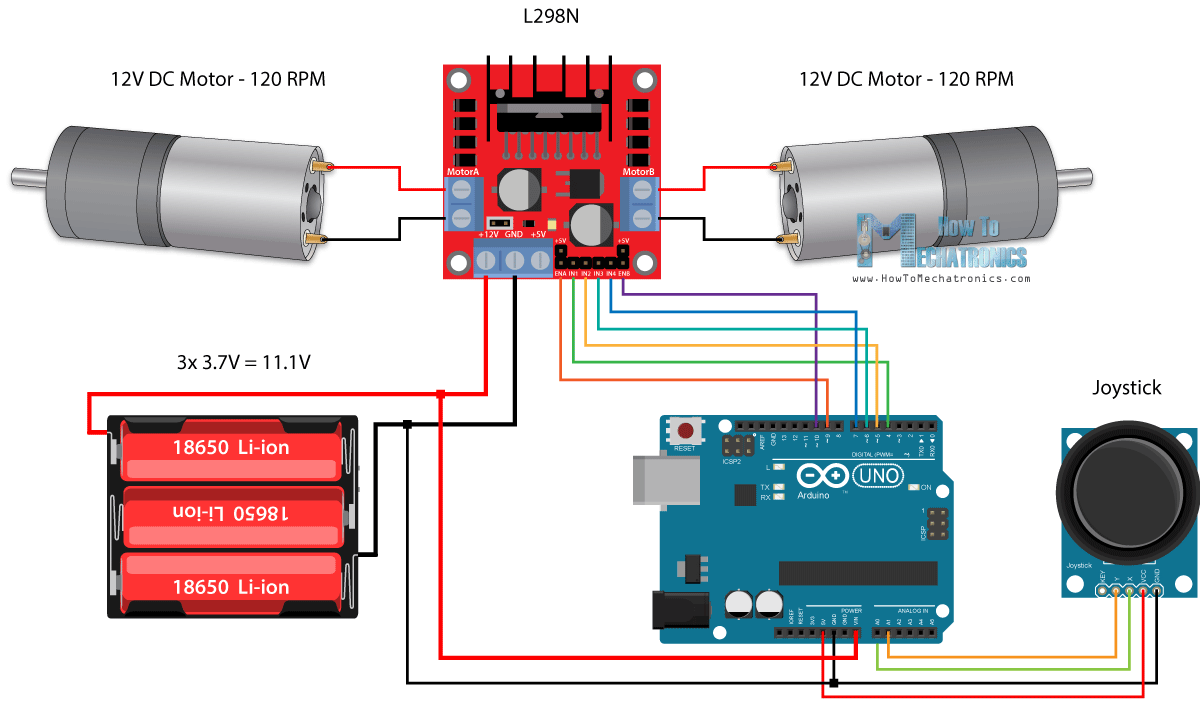
\includegraphics[width=0.5\textwidth]{./img/L298N.png}
\caption{馬達驅動器接線圖}
\label{fig:example}
\end{figure}
\begin{figure}
\centering
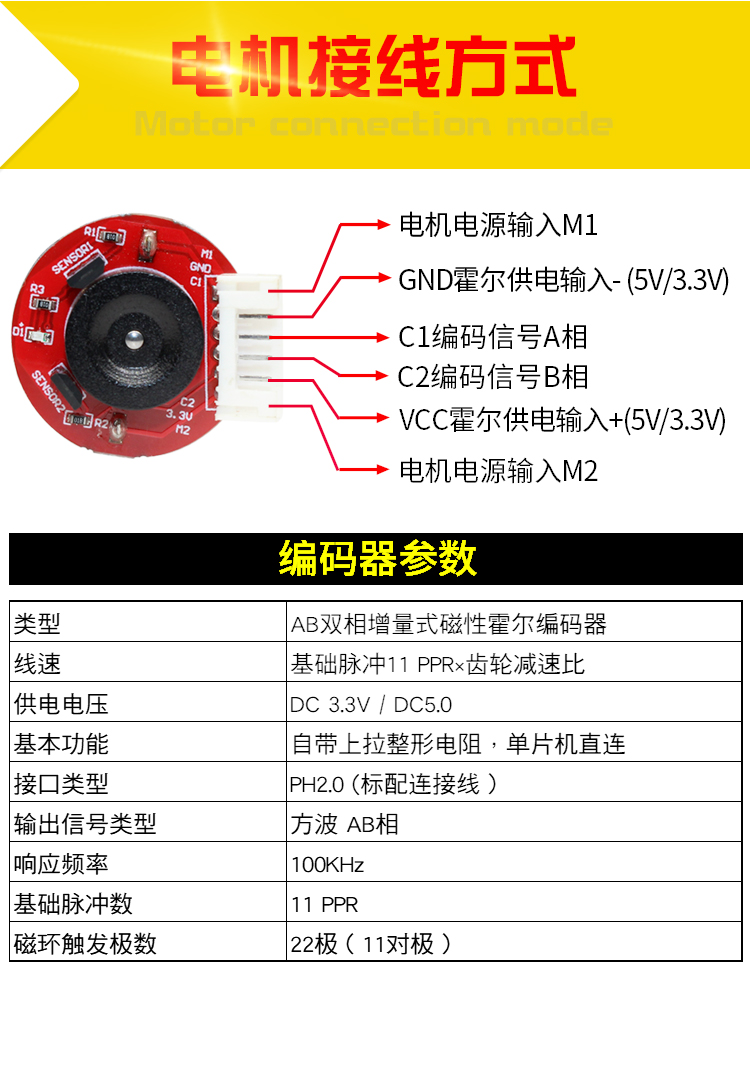
\includegraphics[width=0.5\textwidth]{./img/ZiWcCqr.png}
\caption{霍爾傳感器}
\label{fig:example1}
\end{figure}

\begin{figure}[htp]
\centering
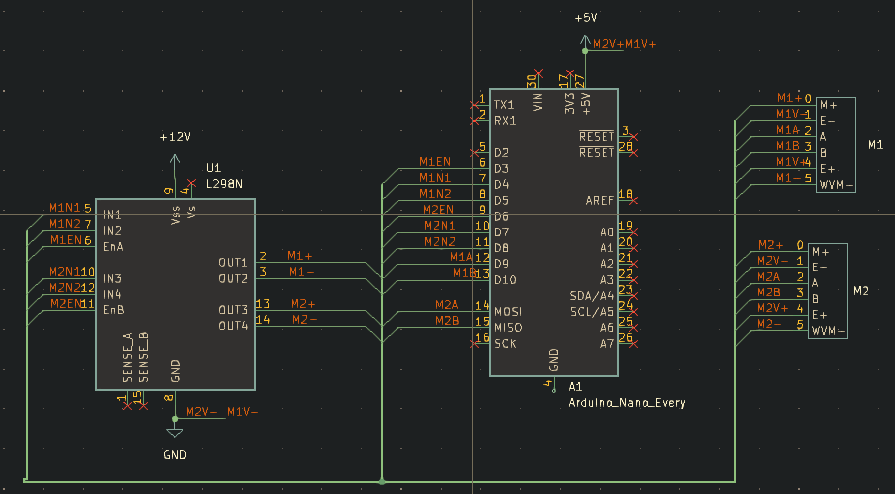
\includegraphics[width=1\textwidth]{./img/arduino.png}
\caption{電路接線圖}
\label{fig:example2}
\end{figure}


\subsection{電路接法}
如圖\ref{fig:example}是驅動器的接線方式,
如圖\ref{fig:example1}是霍爾編碼器的接腳,
圖\ref{fig:example2}是arduino與編碼器跟驅動器的接線圖。
gpio的接腳可以由程式定義,基本上根據定義來接線,IMU的接法如
表\ref{tab:connection}接法一樣之後在把CP2104接到數梅派的USB就
可以用UART通訊讀取資料。


\clearpage
\section{輪子控制}
控制馬達我們要注意的幾個部份
\begin{enumerate}
    \item 控制訊息的格式
    \item arduino 與ros 之間的通訊
    \item PID控制器
    \item 編碼器計算
    \item 里程計計算
\end{enumerate}

\subsection{控制訊息格式}
下面有兩個本次在輪組控制時用到的格式,一個ros內建的用於表示機器在空間中的狀態,
如線性方向的變化(x,y,z)與旋轉變化的(x,y,z),另外一個是我自訂意的變數格式用於表示兩個
輪子的轉動速度(rps)
\begin{itemize}
    \item geometry\_msgs/msg/Twist
    \item diff\_robot\_description/msg/Wheel
\end{itemize}
\begin{tcolorbox}
\begin{verbatim}
ros2 interface show diff_robot_description/msg/Wheel        
--------------------------------------------------------
float64 left_wheel_speed   # 左輪轉速
float64 right_wheel_speed  # 右輪轉速
\end{verbatim}
\end{tcolorbox}
\begin{tcolorbox}
\begin{verbatim}
ros2 interface show geometry_msgs/msg/Twist
-------------------------------------------------------------------------------
# This expresses velocity in free space broken into its linear and angular parts.
Vector3  linear
	float64 x
	float64 y
	float64 z
Vector3  angular
	float64 x
	float64 y
	float64 z
\end{verbatim}
\end{tcolorbox}


\subsection{arduino與ros通訊}
我們這次是用uart通訊來做arduino與ros之間的數據交換。
ros可以用python 的pyserial套件來做urat通訊,arduino用serial就可以了。
\begin{itemize}
    \item ros給arduino目標轉速
    \item arduino給ros測量轉速
\end{itemize}

\subsection{PID}
PID馬達控制透過比例、積分、微分控制器調節馬達輸出,
使實際速度接近目標速度。比例控制速度誤差、
積分控制積累誤差、微分控制速度變化率,綜合調整可達到
精準控制效果。可以參考
\href{https://geekeeceebee.com/index.html}{PID馬達控制}

本次使用
\href{https://github.com/br3ttb/Arduino-PID-Library/tree/master}{arduino pid}
的套件

\begin{itemize}
    \item Setpoint:目標轉速
    \item Input:測量轉速
    \item Output:pwm輸出量
\end{itemize}

\section{輪子控制程式}
輪子本次我們決定用arduino來寫控制程式,其中用uart根ros2通訊,節點如下。
\begin{enumerate}
    \item control\_node 用於訂閱cmd的訊息來轉換成輪子轉速發布給Wheel
    \item Serial 與arduino通訊並把轉速傳給diffodom 
    \item 接收實際轉速換成里程位置
\end{enumerate}

\subsection{control node}
這是一個狀態資訊轉成差速器的節點。Wheel資料是自訂意的資料型態,內容是兩輪的轉速。
\begin{itemize}
    \item 訂閱cmd\_vel
    \item 發布Wheel
    \item 將Twist資料轉成Wheel
\end{itemize}


\subsection{control node python}
\begin{itemize}
    \item $W_r = V+\frac{\omega \times L}{2}$
    \item $W_l = V-\frac{\omega \times L}{2}$
    \begin{itemize}
        \item $W_l$左輪轉速
        \item $W_r$右輪轉速
        \item $L$輪距
        \item $V$前進速度
        \item $\omega$轉彎角速度
    \end{itemize}
\end{itemize}
\begin{lstlisting}[language=Python, caption=control node]
import rclpy
from rclpy.node import Node
from geometry_msgs.msg import Twist
from std_msgs.msg import Float32
from diff_robot_description.msg import Wheel

class ControlNode(Node):
    def __init__(self):
        super().__init__('control_node')
        self.get_logger().info('control node ....')
        self.subscription = self.create_subscription(
            Twist,
            'cmd_vel',
            self.cmd_vel_callback,
            10)
        self.Wheel = self.create_publisher(
            Wheel,
            'Wheel',
            10)
        self.get_logger().info('control node start')

    def cmd_vel_callback(self, msg):
        linear_vel = msg.linear.x
        angular_vel = msg.angular.z
        speed = Wheel()
        L = 0.5
        speed.right_wheel_speed = linear_vel+angular_vel*L/2
        speed.left_wheel_speed  = linear_vel-angular_vel*L/2
        self.get_logger().info('whell:\t%f'%speed.right_wheel_speed)
        self.get_logger().info('left:\t%f'%speed.left_wheel_speed)
        self.Wheel.publish(speed)

def main(args=None):
    rclpy.init(args=args)
    control_node = ControlNode()
    rclpy.spin(control_node)
    control_node.destroy_node()
    rclpy.shutdown()

if __name__ == '__main__':
    main()
\end{lstlisting}
\subsection{serial node(未完成)}
與arduino做通訊目前尚未完工
\begin{lstlisting}[language=Python, caption=control node]
import serial
import rclpy
from rclpy.node import Node
from diff_robot_description.msg import Wheel
class SerialNode(Node):

    def __init__(self):
        super().__init__('serial_node')
        self.publisher_ = self.create_publisher(Wheel, 'Wheel_speed', 10)
        self.subscription = self.create_subscription(
            Wheel,
            'Wheel',
            self.wheel_callback,
            10)
        self.get_logger().info('serial node start')

    def  wheel_callback(self,msg):
        
        self.get_logger().info(str(msg))
        self.get_logger().info('get data:')
        self.publisher_.publish(msg)
        pass
    def serial_get(self):
        Wheel_speed = Wheel
        Wheel_speed.left_wheel_speed = 0.85
        Wheel_speed.right_wheel_speed =0.88

def main(args=None):
    rclpy.init(args=args)
    Serial_Node = SerialNode()
    rclpy.spin(Serial_Node)
    rclpy.shutdown()

if __name__ == '__main__':
    main()
\end{lstlisting}

\subsection{diffodom 里程計計算}
\begin{lstlisting}[language=Python, caption=control node]
from os import walk
import rclpy
from rclpy.node import Node
from diff_robot_description.msg import Wheel
from geometry_msgs.msg import Twist, Vector3
from math import cos, sin
from geometry_msgs.msg import TransformStamped
import tf2_ros
import geometry_msgs.msg

class OdomCalculator(Node):
    def __init__(self):
        super().__init__('odom_calculator')
        self.subscription = self.create_subscription(
            Wheel,
            'Wheel_speed',
            self.wheel_speed_callback,
            10)
        self.publisher = self.create_publisher(
        Twist,
        'odom',
        10)
        self.current_pose = [0.0,0.0,0.0]
        self.tf_broadcaster = tf2_ros.StaticTransformBroadcaster(self)
    def wheel_speed_callback(self,msg):
        left_speed = msg.left_wheel_speed
        right_speed= msg.right_wheel_speed
        wheel_base = 0.5

        linear_vel = (left_speed + right_speed) / 2
        angular_vel = (right_speed - left_speed) / wheel_base
        self.update_odometry(linear_vel, angular_vel)


    def update_odometry(self, linear_vel, angular_vel):
        time_step = 0.1  # 假設時間間隔為0.1秒
        self.current_pose[0] += linear_vel * cos(self.current_pose[2]) * time_step
        self.current_pose[1] += linear_vel * sin(self.current_pose[2]) * time_step
        self.current_pose[2] += angular_vel * time_step
        twist_msg = Twist(
            linear=Vector3(x=self.current_pose[0], y=self.current_pose[1], z=0.0),
            angular=Vector3(x=0.0, y=0.0, z=self.current_pose[2]))
        self.publisher.publish(twist_msg)
        transform_stamped = geometry_msgs.msg.TransformStamped()
        transform_stamped.header.stamp = self.get_clock().now().to_msg()
        transform_stamped.header.frame_id = 'odom'
        transform_stamped.child_frame_id = 'base_link'
        transform_stamped.transform.translation.x = self.current_pose[0]
        transform_stamped.transform.translation.y = self.current_pose[1]
        transform_stamped.transform.rotation.w = cos(self.current_pose[2] / 2)
        transform_stamped.transform.rotation.x = 0.0
        transform_stamped.transform.rotation.y = 0.0
        transform_stamped.transform.rotation.z = sin(self.current_pose[2] / 2)

        self.tf_broadcaster.sendTransform(transform_stamped)
      

def main(args=None):
    rclpy.init(args=args)
    odom_calculator = OdomCalculator()
    rclpy.spin(odom_calculator)
    odom_calculator.destroy_node()
    rclpy.shutdown()


if __name__ == '__main__':
    main()

\end{lstlisting}



\section{里程記設定}
再有編碼器的情況下我們就可以計算我們的移動距離與轉向。
相關的之料可以提供給導航模組去使用。

\section{導航設定}
這部份我還沒研究完,我看dblanding大大這部份只有寫參數設定,根
啟動檔,這邊應該除了dblanding的github還要在查看其他資料。
\subsection{導航參數文件}
\begin{table}[ht]
\centering
\begin{tabularx}{\textwidth}{|l|X|}
\hline
\textbf{檔案名稱}                     & \textbf{用途}                                                   \\ \hline
base\_local\_planner\_params.yaml  & 配置基礎局部規劃器(local planner)的參數                         \\ \hline
costmap\_common\_params.yaml       & 配置共用的地圖(costmap)參數,用於全局和局部 costmap             \\ \hline
dwa\_local\_planner\_params.yaml   & 配置動態窗口局部規劃器(Dynamic Window Approach)的參數         \\ \hline
global\_costmap\_params.yaml       & 配置全局 costmap 的參數                                         \\ \hline
global\_planner\_params.yaml       & 配置全局規劃器(global planner)的參數                           \\ \hline
local\_costmap\_params.yaml        & 配置局部 costmap 的參數                                         \\ \hline
move\_base\_params.yaml            & 配置 move\_base 模組的參數,用於整合全局和局部規劃器以及 costmap \\ \hline
navfn\_global\_planner\_params.yaml& 配置基於 Dijkstra 或 A* 算法的全局規劃器(navfn)的參數          \\ \hline
\end{tabularx}
\end{table}



\clearpage
\section{參數設定}
參數如下


\section{啟動檔}


\section{SLAM Toolbox}
SLAM Toolbox: 這是一個用於ROS 2的SLAM解決方案,用於構建
機器人周圍環境的地圖並同時估計機器人的位置。SLAM Toolbox
通常會生成一個地圖,描述了機器人周圍的環境,並用於
後續的導航任務。


\begin{tcolorbox}
\begin{verbatim}
ros2 pkg executables slam_toolbox
----------------------------------
slam_toolbox async_slam_toolbox_node
slam_toolbox localization_slam_toolbox_node
slam_toolbox map_and_localization_slam_toolbox_node
slam_toolbox merge_maps_kinematic
slam_toolbox sync_slam_toolbox_node
\end{verbatim}
\end{tcolorbox}
\begin{enumerate}
    \item async\_slam\_toolbox\_node: 非同步SLAM節點,用於接收激光雷達數據並建構地圖,同時估計機器人的位置。這個節點可以在SLAM過程中非同步地處理數據,提高了效率。
    \item localization\_slam\_toolbox\_node: 定位節點,用於在已知地圖的情況下估計機器人的位置。這個節點通常用於在已經建立好地圖的環境中進行機器人定位。
    \item map\_and\_localization\_slam\_toolbox\_node: 地圖和定位節點,結合了地圖建構和定位功能。這個節點可以同時建構地圖並估計機器人的位置,適用於需要即時定位和地圖更新的場景。
    \item merge\_maps\_kinematic: 地圖合併工具,用於將多個地圖合併成一個更大的地圖。這個工具可以用於將不同時間或不同地點生成的地圖合併成一個整體地圖。
    \item sync\_slam\_toolbox\_node: 同步SLAM節點,類似於非同步SLAM節點,用於接收激光雷達數據並建構地圖,但在處理數據時採用同步方式,可以更精確地估計機器人的位置。
\end{enumerate}
\subsection{slam toolbox節點訊息}
async\_slam\_toolbox\_node只有一個節點slam toolbox,
他的訊息如下

\begin{itemize}
    \item 訂閱者(Subscribers):
    \begin{itemize}
        \item /map:接收地圖資料 (nav\_msgs/msg/OccupancyGrid)。
        \item /parameter\_events:接收參數事件 (rcl\_interfaces/msg/ParameterEvent)。
        \item /scan:接收雷射掃描資料 (sensor\_msgs/msg/LaserScan)。
        \item /slam\_toolbox/feedback:接收互動標記反饋 \\
            (visualization\_msgs/msg/InteractiveMarkerFeedback)。
    \end{itemize}
    \item 發布者(Publishers):
    \begin{itemize}
        \item /map:發布地圖資料 (nav\_msgs/msg/OccupancyGrid)。
        \item /map\_metadata:發布地圖的元資料 (nav\_msgs/msg/MapMetaData)。
        \item /parameter\_events:發布參數事件 (rcl\_interfaces/msg/ParameterEvent)。
        \item /pose:發布具有協方差的姿態資訊 (geometry\_msgs/msg/PoseWithCovarianceStamped)。
        \item /rosout:用於 ROS 輸出 \\
            (rcl\_interfaces/msg/Log)。
        \item /slam\_toolbox/graph\_visualization:發布圖形可視化資料\\
            (visualization\_msgs/msg/MarkerArray)。
        \item /slam\_toolbox/scan\_visualization:發布雷射掃描資料的可視化 (sensor\_msgs/msg/LaserScan)。
        \item /slam\_toolbox/update:用於更新互動標記的訊息 
            \\(visualization\_msgs/msg/InteractiveMarkerUpdate)。
        \item /tf:發布 TF 訊息 (tf2\_msgs/msg/TFMessage)。
    \end{itemize}
    \item 服務伺服器(Service Servers):
    \begin{itemize}
        \item /slam\_toolbox/clear\_changes:用於清除變更的服務 \\
            (slam\_toolbox/srv/Clear)。
        \item /slam\_toolbox/describe\_parameters:用於描述參數的服務 
            \\(rcl\_interfaces/srv/DescribeParameters)。
        \item /slam\_toolbox/deserialize\_map:用於反序列化地圖的服務 
            \\(slam\_toolbox/srv/DeserializePoseGraph)。
        \item /slam\_toolbox/dynamic\_map:用於獲取動態地圖的服務 
            \\(nav\_msgs/srv/GetMap)。
        \item /slam\_toolbox/get\_interactive\_markers:用於獲取互動標記的服務 
            \\(visualization\_msgs/srv/GetInteractiveMarkers)。
        \item /slam\_toolbox/get\_parameter\_types:用於獲取參數類型的服務 
            \\(rcl\_interfaces/srv/GetParameterTypes)。
        \item /slam\_toolbox/get\_parameters:用於獲取參數的服務 
            \\(rcl\_interfaces/srv/GetParameters)。
        \item /slam\_toolbox/list\_parameters:用於列出參數的服務 
            \\(rcl\_interfaces/srv/ListParameters)。
        \item /slam\_toolbox/manual\_loop\_closure:用於手動閉環的服務 
            \\(slam\_toolbox/srv/LoopClosure)。
        \item /slam\_toolbox/pause\_new\_measurements:用於暫停新測量的服務 (slam\_toolbox/srv/Pause)。
        \item /slam\_toolbox/save\_map:用於保存地圖的服務 (slam\_toolbox/srv/SaveMap)。
        \item /slam\_toolbox/serialize\_map:用於序列化地圖的服務 (slam\_toolbox/srv/SerializePoseGraph)。
        \item /slam\_toolbox/set\_parameters:用於設置參數的服務 (rcl\_interfaces/srv/SetParameters)。
        \item /slam\_toolbox/set\_parameters\_atomically:用於原子設置參數的服務 
            \\(rcl\_interfaces/srv/SetParametersAtomically)。
        \item /slam\_toolbox/toggle\_interactive\_mode:用於切換互動模式的服務 
            \\(slam\_toolbox/srv/ToggleInteractive)。
    \end{itemize}
\end{itemize}
提供一系列服務,包括清除變化、描述參數、反序列化地圖、獲取動態地圖、獲取互動式標記等。

\subsubsection{topic節點}
上面的節點就可以看得出來他的topic很多。

\begin{itemize}
    \item /joint\_states: 發布機器人各個關節的狀態,包括位置、速度等信息,通常由機器人的控制器發布。
    \item /map: SLAM(同步定位與地圖構建)算法生成的地圖,通常是一個佔用格地圖(Occupancy Grid Map),描述了機器人周圍的環境。
    \item /map\_metadata: 地圖的元數據,包含了地圖的尺寸、分辨率等信息。
    \item /parameter\_events: 發布參數的變更事件,用於通知參數發生了變化。
    \item /pose: 發布機器人的姿態信息,包括位置和方向。
    \item /robot\_description: 包含了機器人的URDF(Unified Robot Description Format)描述,用於描述機器人的結構和幾何形狀。
    \item /rosout: ROS系統的輸出信息,包括日誌和調試信息。
    \item /scan: 激光雷達的掃描數據,用於感測機器人周圍的障礙物。
    \item /slam\_toolbox/feedback: 互動標記的反饋信息,用於顯示和操作地圖上的互動標記。
    \item /slam\_toolbox/graph\_visualization: 圖形可視化數據,用於在地圖上顯示標記或軌跡等信息。
    \item /slam\_toolbox/scan\_visualization: 激光雷達數據的可視化,用於在RViz等工具中顯示激光雷達掃描。
    \item /slam\_toolbox/update: 更新互動標記的消息,用於更新地圖上的互動標記。
    \item /tf: 用於傳遞坐標變換信息,描述了不同坐標系之間的關係。
    \item /tf\_static: 用於傳遞靜態的坐標變換信息,這些變換在運行時不會改變。
\end{itemize}

\subsubsection{參數}

\begin{itemize}
    \item angle\_variance\_penalty: 角度變異懲罰。

    \item base\_frame: 機器人的基礎座標系。

    \item ceres\_dogleg\_type: Ceres解算器的Dogleg類型。

    \item ceres\_linear\_solver: Ceres解算器的線性求解器。

    \item ceres\_loss\_function: Ceres解算器的損失函數。

    \item ceres\_preconditioner: Ceres解算器的預處理器。

    \item ceres\_trust\_strategy: Ceres解算器的信任策略。

    \item coarse\_angle\_resolution: 粗糙角度解析度。

    \item coarse\_search\_angle\_offset: 粗糙搜索角度偏移量。

    \item correlation\_search\_space\_dimension: 相關性搜索空間維度。

    \item correlation\_search\_space\_resolution: 相關性搜索空間解析度。

    \item correlation\_search\_space\_smear\_deviation: 相關性搜索空間模糊偏差。

    \item debug\_logging: 調試日誌記錄。

    \item distance\_variance\_penalty: 距離方差懲罰。

    \item do\_loop\_closing: 是否執行循環閉合。

    \item enable\_interactive\_mode: 是否啟用互動模式。

    \item fine\_search\_angle\_offset: 精細搜索角度偏移量。

    \item interactive\_mode: 互動模式。

    \item link\_match\_minimum\_response\_fine: 連接匹配最小響應(細)。

    \item link\_scan\_maximum\_distance: 連接掃描最大距離。

    \item loop\_match\_maximum\_variance\_coarse: 循環匹配最大方差(粗)。

    \item loop\_match\_minimum\_chain\_size: 循環匹配最小鏈尺寸。

    \item loop\_match\_minimum\_response\_coarse: 循環匹配最小響應(粗)。

    \item loop\_match\_minimum\_response\_fine: 循環匹配最小響應(細)。

    \item loop\_search\_maximum\_distance: 循環搜索最大距離。

    \item loop\_search\_space\_dimension: 循環搜索空間維度。

    \item loop\_search\_space\_resolution: 循環搜索空間解析度。

    \item loop\_search\_space\_smear\_deviation: 循環搜索空間模糊偏差。

    \item map\_file\_name: 地圖檔案名稱。

    \item map\_frame: 地圖座標系。

    \item map\_name: 地圖名稱。

    \item map\_start\_at\_dock: 地圖是否從碼頭開始。

    \item map\_start\_pose: 地圖的起始姿態。

    \item map\_update\_interval: 地圖更新間隔。

    \item minimum\_angle\_penalty: 最小角度懲罰。

    \item minimum\_distance\_penalty: 最小距離懲罰。

    \item minimum\_time\_interval: 最小時間間隔。

    \item minimum\_travel\_distance: 最小行駛距離。

    \item minimum\_travel\_heading: 最小行駛方向。

    \item mode: 模式(地圖構建或定位)。

    \item odom\_frame: 里程計座標系。

    \item paused\_new\_measurements: 暫停新測量。

    \item paused\_processing: 暫停處理。

    \item position\_covariance\_scale: 位置協方差比例。

    \item qos\_overrides: QoS覆蓋。

    \item resolution: 解析度。

    \item scan\_buffer\_maximum\_scan\_distance: 掃描緩衝區最大掃描距離。

    \item scan\_buffer\_size: 掃描緩衝區大小。

    \item scan\_queue\_size: 掃描隊列大小。

    \item scan\_topic: 掃描主題。

    \item solver\_plugin: 解算器插件。

    \item tf\_buffer\_duration: TF緩衝區持續時間。

    \item throttle\_scans: 掃描節流。

    \item transform\_publish\_period: 變換發布週期。

    \item transform\_timeout: 變換超時。

    \item use\_map\_saver: 是否使用地圖保存器。

    \item use\_response\_expansion: 是否使用響應擴展。

    \item use\_scan\_barycenter: 是否使用掃描重心。

    \item use\_scan\_matching: 是否使用掃描匹配。

    \item use\_sim\_time: 是否使用模擬時間。

    \item yaw\_covariance\_scale: 偏航協方差比例。
\end{itemize}

\section{lidar}

\subsection{操作方法}

本次使的lidar是RPLIDAR-A1,再有ros2的套件輔助下我們可以教簡
單使用。
\begin{enumerate}
    \item 使用git把原始碼安裝在工作目錄
    \item 編譯原始碼
    \item 執行測試
\end{enumerate}
\subsubsection{安裝編譯原始碼}
動作流程如下。
\begin{tcolorbox}
\begin{verbatim}
    cd ~/ros2_ws/src
    git clone https://github.com/Slamtec/sllidar_ros2
    cd ../ 
    rosdep install -i --from-path src --rosdistro humble -y
    colcon build --packages-select sllidar_ros2
\end{verbatim}
\end{tcolorbox}
\begin{enumerate}
    \item 移動到工作目錄的原始碼資料夾
    \item 下載lidar的套件
    \item 回到工作根目錄
    \item 檢查相依程式
    \item 開始編譯
\end{enumerate}
\subsubsection{測試與使用}
編譯完原始碼的話基本上就可以使用了,使用方法如下
\begin{tcolorbox}
\begin{verbatim}
    source install/setup.zsh    
    ros2 launch sllidar_ros2 sllidar_a1_launch.py
    #可以選折下面有視覺化設定的
    ros2 launch sllidar_ros2 view_sllidar_a1_launch.py
\end{verbatim}
\end{tcolorbox}
\begin{enumerate}
    \item 啟用ros2環境
    \item 開啟lidar的請動檔
\end{enumerate}
這邊要注意使用的光達型號不同型號有對應的啟動檔,也可以直接
使用可是化的啟動檔view開頭的那個。
\subsection{檢視資料}
接下來就以觀察這個套件有哪些要注意的地方。

\begin{itemize}
    \item 開啟的節點
    \item 主題的發布與訂閱
    \item 資料的格式
    \item 節點參數
\end{itemize}
\subsubsection{節點說明}
這個光達啟動檔產生的節點為/sllidar\_node,我們可以用info查
詢相關訊息。
\begin{tcolorbox}
\begin{verbatim}
    ros2 node info /sllidar\_node
\end{verbatim}
\end{tcolorbox}
這樣可以看到下面有關node的通訊狀況,包含他會訂閱/發布哪些主
題與服務根動作。
\begin{itemize}
    \item 訂閱器(Subscribers):
        \begin{itemize}
            \item /parameter\_events:訂閱參數事件的消息,
                類型為 rcl\_interfaces/msg/ParameterEvent。
        \end{itemize}
    \item 發布器(Publishers):

        \begin{itemize}
            \item /parameter\_events:發布參數事件的消息,
                類型為 rcl\_interfaces/msg/ParameterEvent。
            \item /rosout:發布ROS的日誌消息,類型為 
                rcl\_interfaces/msg/Log。
            \item /scan:發布激光雷達掃描消息,類型為 
                sensor\_msgs/msg/LaserScan。
        \end{itemize}
    \item 服務伺服器(Service Servers):
        \begin{itemize}
            \item /sllidar\_node/describe\_parameters:提供描
                述參數的服務,類型為 \\
                rcl\_interfaces/srv/DescribeParameters。
            \item /sllidar\_node/get\_parameter\_types:提供獲
                取參數類型的服務,類型為 \\
                rcl\_interfaces/srv/GetParameterTypes。
            \item /sllidar\_node/get\_parameters:提供獲取參數
                值的服務,類型為 \\
                rcl\_interfaces/srv/GetParameters。
            \item /sllidar\_node/list\_parameters:
                提供列出參數的服務,類型為\\
                rcl\_interfaces/srv/ListParameters。
            \item /sllidar\_node/set\_parameters:
                提供設置參數值的服務,類型為 \\
                rcl\_interfaces/srv/SetParameters。
            \item /sllidar\_node/set\_parameters\_atomically:
                提供原子設置多個參數值的服務,類型為 \\
                rcl\_interfaces/srv/SetParametersAtomically。
            \item /start\_motor:提供啟動馬達的服務,
                類型為 std\_srvs/srv/Empty。
            \item /stop\_motor:提供停止馬達的服務,類型為 
                std\_srvs/srv/Empty。
        \end{itemize}
    \item 服務客戶端(Service Clients):(未提供)
    \item 動作伺服器(Action Servers):(未提供)
    \item 動作客戶端(Action Clients):(未提供)
\end{itemize}

這些功能使得sllidar\_node節點能夠與其他節點進行通訊和交互操作,從而實現控制和獲取激光雷達的功能。

\subsubsection{topic查詢}
首先要確認/scan的訊息。
\begin{tcolorbox}
\begin{verbatim}
    ros2 lidar info /scan
------------------------------------------
Type: sensor_msgs/msg/LaserScan
Publisher count: 1
Subscription count: 0
\end{verbatim}
\end{tcolorbox}
我們看得出來他的,訂閱與發不的狀況根他的數據界面。
再來我們可以用echo來監聽這個主題。
\begin{tcolorbox}
\begin{verbatim}
    ros2 topic echo /scan --once
-----------------------------------
    header:
  stamp:
    sec: 1710051588
    nanosec: 187130763
  frame_id: laser
angle_min: -3.1241390705108643
angle_max: 3.1415927410125732
angle_increment: 0.005806980188935995
time_increment: 0.0001362734183203429
scan_time: 0.1470390260219574
range_min: 0.15000000596046448
range_max: 12.0
ranges:
.......
intensities:
\end{verbatim}
\end{tcolorbox}
有關各個數值的意義如下
\begin{itemize}
    \item header:包含時間戳記(stamp)和框架 ID(frame\_id),用於確定訊息的時間和座標系。
    \item stamp:時間戳記,以秒(sec)和納秒(nanosec)表示。
    \item frame\_id:訊息的座標系標識符,在這裡是 laser。
    \item angle\_min:激光雷達掃描的最小角度(弧度)。
    \item angle\_max:激光雷達掃描的最大角度(弧度)。
    \item angle\_increment:每個激光束之間的角度增量(弧度)。
    \item time\_increment:每個激光束的時間增量(秒)。
    \item scan\_time:完成一次完整掃描所需的時間(秒)。
    \item range\_min:激光雷達能夠測量的最小距離(公尺)。
    \item range\_max:激光雷達能夠測量的最大距離(公尺)。
    \item ranges:每個激光束測量的距離值陣列。
    \item intensities:每個激光束的強度值陣列(有些激光雷達可以測量強度,但並非所有)。
\end{itemize}
\subsubsection{參數查詢}
接下來就是參數的訊息了,透過param dump來查看

\begin{tcolorbox}
\begin{verbatim}
    ros2 param dump /sllidar_node
-------------------------------------------
/sllidar_node:
  ros__parameters:
    angle_compensate: true
    channel_type: serial
    frame_id: laser
    inverted: false
    qos_overrides:
      /parameter_events:
        publisher:
          depth: 1000
          durability: volatile
          history: keep_last
          reliability: reliable
    scan_frequency: 10.0
    scan_mode: ''
    serial_baudrate: 115200
    serial_port: /dev/ttyUSB0
    tcp_ip: 192.168.0.7
    tcp_port: 20108
    udp_ip: 192.168.11.2
    udp_port: 8089
    use_sim_time: false
\end{verbatim}
\end{tcolorbox}
這是sllidar\_node節點的參數設定。讓我們逐個解釋:
\begin{enumerate}
    \item angle\_compensate:角度補償,設置為true表示啟用角度補償。
    \item channel\_type:通道類型,這裡設置為serial。
    \item frame\_id:訊息的座標系標識符,在這裡是laser。
    \item inverted:是否反向,設置為false表示不反向。
    \item qos\_overrides:QoS覆蓋設定,這裡設置了一些QoS參數。
    \item scan\_frequency:掃描頻率,設置為10.0 Hz。
    \item serial\_baudrate:串口波特率,設置為115200。
    \item serial\_port:串口端口,設置為/dev/ttyUSB0。
    \item tcp\_ip:TCP IP地址,設置為192.168.0.7。
    \item tcp\_port:TCP端口,設置為20108。
    \item udp\_ip:UDP IP地址,設置為192.168.11.2。
    \item udp\_port:UDP端口,設置為8089。
    \item use\_sim\_time:使用模擬時間,設置為false表示不使用模擬時間。
\end{enumerate}

這些參數描述了sllidar\_node節點的配置,包括通訊方式、座標
系、掃描頻率等,我們是走serial通訊的,所以要
注意port的參數未來接上的設定。

\subsection{資料視覺化}
這裡我們用rviz可以更清楚的看到光達所掃掉的資料。

\begin{enumerate}
    \item 打開終端機
    \item 輸入rviz2
    \item 設定fixed frame = laser
    \item 在add加入laser scan的資料
\end{enumerate}

\section{yolov8辨識}
ros2 有yolov8的套件可以用
\href{https://github.com/mgonzs13/yolov8_ros/tree/main}{yolov8\_ros}。
\subsection{安裝方法}
流程如下,就照指令做就好了。
\begin{tcolorbox}
\begin{verbatim}
 cd ~/ros2_ws/src
 git clone https://github.com/mgonzs13/yolov8_ros.git
 pip3 install -r yolov8_ros/requirements.txt
 cd ~/ros2_ws
 rosdep install --from-paths src --ignore-src -r -y
 colcon build
\end{verbatim}
\end{tcolorbox}
\subsection{基本操作}
\begin{tcolorbox}
\begin{verbatim}
$ ros2 launch yolov8_bringup yolov8.launch.py
\end{verbatim}
\end{tcolorbox}
\subsection{主題與參數}
\begin{itemize}
    \item Topics
    \begin{itemize}
        \item /yolo/detections: Objects detected by YOLO using the RGB images. Each object contains a bounding boxes and a class name. It may also include a mak or a list of keypoints.
        \item /yolo/tracking: Objects detected and tracked from YOLO results. Each object is assigned a tracking ID.
        \item /yolo/debug\_image: Debug images showing the detected and tracked objects. They can be visualized with rviz2.
    \end{itemize}
    \item Parameters
    \begin{itemize}
        \item model: YOLOv8 model (default: yolov8m.pt)
        \item tracker: Tracker file (default: bytetrack.yaml)
        \item device: GPU/CUDA (default: cuda:0)
        \item enable: Wether to start YOLOv8 enabled (default: True)
        \item threshold: Detection threshold (default: 0.5)
        \item input\_image\_topic: Camera topic of RGB images (default: /camera/rgb/image\_raw)
        \item  image\_reliability: Reliability for the image topic: 0=system default, 1=Reliable, 2=Best Effort (default: 2)
    \end{itemize}
\end{itemize}
\subsection{注意事項}
使用時他會去訂閱/camera/rgb/image\_raw的topic所以要把想要做辨識的圖發布到這裡。

\subsection{程式分析}
\subsubsection{yolov8\_node.py}

這段程式碼是一個 ROS 2 節點,用於在圖像中偵測和追蹤物體,並且發布偵測到的物體資訊。
節點使用 YOLOv8 模型進行物體偵測,並透過 ROS 2 訊息將偵測到的物體發布出去。

該節點繼承自 LifecycleNode 類別,實現了節點的生命週期方法
(on\_configure、on\_activate、\\ on\_deactivate、on\_cleanup),
並實現了 enable\_cb 方法來處理啟用/禁用節點的服務請求。
節點還實現了一些輔助方法來解析 YOLOv8 的偵測結果,並將結果轉換為 ROS 2 訊息。

在 main 函數中,節點初始化後手動觸發了配置和啟用操作,
並通過 rclpy.spin(node) 來啟動節點的訊息迴圈,等待訊息的到來和處理。\href{https://github.com/mgonzs13/yolov8_ros/blob/main/yolov8_ros/yolov8_ros/yolov8_node.py}{src}


\begin{itemize}
    \item \_\_init\_\_(self, **kwargs) 
        None: 初始化函式,用於初始化節點的各種參數和屬性。
    \item on\_configure(self, state: LifecycleState) \\
        TransitionCallbackReturn: 配置函式,用於配置節點在啟動前的相關設置。
    \item enable\_cb(self, request, response): 啟用/禁用節點的服務回調函式。
    \item on\_activate(self, state: LifecycleState) \\
        TransitionCallbackReturn: 啟動函式,用於啟動節點並開始執行相應的任務。
    \item on\_deactivate(self, state: LifecycleState) \\
        TransitionCallbackReturn: 停用函式,用於停用節點並進行清理工作。
    \item on\_cleanup(self, state: LifecycleState) \\
        TransitionCallbackReturn: 清理函式,用於在節點結束運行時進行清理工作。
    \item parse\_hypothesis(self, results: Results) \\
        List[Dict]: 解析假設的函式,用於解析物體偵測的結果,返回一個假設列表。
    \item parse\_boxes(self, results: Results)\\
         List[BoundingBox2D]: 解析框框的函式,用於解析物體偵測的結果,返回一個框框列表。
    \item parse\_masks(self, results: Results) \\
        List[Mask]: 解析遮罩的函式,用於解析物體偵測的結果,返回一個遮罩列表。
    \item parse\_keypoints(self, results: Results) \\
        List[KeyPoint2DArray]: 解析關鍵點的函式,用於解析物體偵測的結果,返回一個關鍵點列表。
    \item image\_cb(self, msg: Image) \\
        None: 圖像回調函式,用於接收來自訂閱的圖像訊息並進行物體偵測處理
\end{itemize}



\section{實做紀錄}

\subsection{2-25 到 3-02}
本週拿到jetson nano了。
\begin{itemize}
    \item jetson nano
\end{itemize}
\subsubsection{完成任務}
本週住要將jection的作業環境搭建完成,只是nvidia提供的版本
是,ubuntu18.04的版本這不是我們要的版本,所以提升到22.04
但是應為套件的關西更新根升級的時間會花很久。
\begin{itemize}
    \item 安裝 jetpack4.6板
    \item 將內部作業系統升級22.04
    \item usb 與ssh通訊測試
    \item 完成3D列硬的參數測試
\end{itemize}
\subsubsection{遇到的困難}
jetson nano已經停產,所以nvidia沒有為nano做軟體的更新服務
所以jetpack可以用的版本停在4.6板,再上去的版本沒有直接
支援,但這部份只是光方沒寫支援實際我還沒測過,本次的作法
是用jetpack4.6內的ubuntu18.04直接升級到22.04,目前還沒遇到
兼容性問題。
\begin{itemize}
    \item nvidia 軟體支援差
\end{itemize}

\subsection{3-3 到 3-9}
這周零件陸陸續續的收到了,現在手邊的東西有。

\begin{itemize}
    \item 光達
    \item 馬達驅動器
    \item jetson nano
        n nano以今停產,
    \item 不斷電系統
    \item imu 
    \item 航空電池
    \item usb to ttl
    \item 輪子
\end{itemize}

\subsubsection{完成任務}
這周主要收到光達,以測試光達為主。

\subsubsection{遇到的困難}
剛開始的時候雖然官方有提供驅動,所以輕鬆的可以看到/scan
的訊息,但是我在rviz2上只能在laser上看到訊號,在其他座標
係就看不到了,這主要是我的tf觀念有問題要。

\begin{itemize}
    \item 注意tf id
    \item 靜態廣播
    \item urdf設定
\end{itemize}
\subsection{3-10 到 3-14}
\begin{itemize}
    \item if 樹設定
    \item urdf模型設定
\end{itemize}
\subsection{3-15 到 3-21}
\begin{itemize}
    \item 光學雷達里程計 
    \item slam 製圖
\end{itemize}
\subsection{3-22 到 3-28}
\begin{itemize}
    \item 確認馬達相關參數
    \item ros2馬達控制節點
    \item ros2馬達serial節點
    \item ros2馬達里程節點
\end{itemize}

\section{4月實做紀錄}
\subsection{401到407}
輪組的材料檢查
\begin{itemize}
    \item 確認接線方法
    \item 設計個模組間的接線
\end{itemize}
\subsection{408到414}
完成了輪子編碼器設定,馬達的轉速測量
\begin{itemize}
    \item 完成輪組控制電路
    \item 測量控制訊號
    \item 測量霍爾編碼器訊號
\end{itemize}
\subsection{415到421}
本週期中考基本上沒有進度,主裝材料改成用材料行的盒子。
\begin{itemize}
    \item 完成pid調整
    \item 完成輪組控制鐵三角(目標、控制、里程)
    \item 3d列硬大失敗
    \item 修改外觀材料
\end{itemize}
\subsection{422到428}
以完成基本的框架,現在可以進行基本的控制slam與導航。
\begin{itemize}
    \item 車子的前後左右的控制
    \item 光達的slam製圖
    \item nav2導航
\end{itemize}

\subsubsection{問題}
還是jetson的兼容問題,主要是官方沒有提供22.04的版本所以我們從官方提供的最新18.04進行
升級,但是還是有某些軟體不會跟著所以再把我筆點的程式與ros2的套件轉移到jetson nano來
運作時就時常會有軟體相依性的問題。

再來可能是官方已經擺爛了所以20.04或是往後感覺他的驅動都可能會有問題,這次arduino nano
在根jetson nano 做uart的通訊時,也出現亂碼很明縣就是有大量的雜訊干擾雖然反覆的交叉
比對之後最後有把通訊問題排除。

usb wifi 非常不穩定,我在用ssh登入jetson時很卡並且運算上感覺不是很好。




\end{document}
